\subsection{Inteligencia Artificial}

La Inteligencia Artificial es la inteligencia llevado a cabo por máquinas en las que una máquina “inteligente” ideal es un agente flexible que percibe su entorno y lleva a cabo acciones que maximicen sus posibilidades de éxito en algún objetivo \parencite{tec_poole1998machinelearning}. Este término se aplica cuando una máquina imita las funciones “cognitivas” que asocian los humanos con otras mentes \parencite{bk_russell2009intart}.

Durante la historia de la humanidad, se han seguido 4 enfoques: dos centrados en el comportamiento humano y dos enfocados en torno a la racionalidad. El enfoque centrado en el comportamiento humano se basa en una ciencia empírica, es decir, mediante experimentos que incluyen hipótesis y confirmaciones. Este enfoque nace a partir de la prueba de Alan Turing, en 1950, en la cual, el célebre matemático inglés diseñó una prueba basada en la incapacidad de diferenciar entre entidades inteligentes indiscutibles y seres humanos por parte de un computador. Si este era capaz de diferenciar y superar la prueba mientras que el humano no, se afirma que se trataba de una “máquina inteligente”. Por ello, el computador debía contar con las siguientes capacidades: procesamiento de lenguaje natural para poder comunicarse, representación del conocimiento describiendo lo que percibe de su entorno, razonamiento automático utilizando la información procesada en su interior, y aprendizaje automático para adaptarse a nuevos eventos. Si el evaluador decide incluir una señal de video para evaluar la percepción de la computadora, se dice que se está realizando la Prueba Global de Turing. Para superarla, además de las 4 anteriormente mencionadas, la computadora debe contar además con las capacidades de visión computacional para percibir objetos y robótica con el fin de manipularlos. Todas estas seis capacidades o disciplinas abarcan la mayor parte de la Inteligencia Artificial \parencite{bk_russell2004intart}.

Por el otro lado, el enfoque racional implica una combinación de ingeniería y matemáticas basándose en las “leyes del pensamiento”. Estas parten de la Grecia antigua, planteadas por grandes filósofos como Aristóteles en su intento de codificar la “manera correcta de pensar”, lo que más adelante derivó al estudio de la lógica. Más adelante, en el siglo XIX, se construyeron programas capaces de resolver problemas en notación lógica. De ahí que la tradición logista dentro del campo de la Inteligencia Artificial trata de construir sistemas inteligentes con estas capacidades. De todo lo anterior dicho respecto al enfoque racional se creó el término de un agente racional, el cual actúa intentando lograr el mejor resultado, o de existir incertidumbre, el mejor resultado esperado. Finalmente, la amplia aplicación de la Inteligencia Artificial y sus fundamentos derivan en muchas ciencias de las cuales se pueden mencionar, además de la filosofía y las matemáticas, a la economía, neurociencia, psicología, la ingeniería computacional, la teoría de control y cibernética, y hasta la lingüística \parencite{bk_russell2004intart}.

Pero, ¿cómo es surge este amplio estudio de la Inteligencia Artificial? En 1943, basándose en la fisiología básica y funcionamiento de las neuronas en el cerebro, el análisis formal de la lógica proposicional de Russell y Whitehead, y la teoría computacional de Turing, dos estudiosos en neurociencia realizaron juntos el que sería considerado primer trabajo de Inteligencia Artificial. Warren McCulloch y Walter Pitts propusieron un modelo constituido por neuronas artificiales, en el que cada una de ellas se caracterizaba por estar “activada” o “desactivada”; la del primer tipo daba como resultado a la estimulación producida por una cantidad suficiente de neuronas vecinas. Como ejemplo, mostraron que cualquier función de cómputo podría calcularse mediante alguna red de neuronas interconectadas y que todos los conectores lógicos eran capaces de ser implementados usando estructuras sencillas de red. Seis años más adelante, Donald Hebb propuso una regla de actualización de intensidades de conexiones entre las neuronas, la que actualmente se le conoce como la “regla de aprendizaje Hebbiano” vigente hasta nuestros días. En 1956, Allen Newell y Herbert Simon inventaron un programa de computación en el taller de Dartmouth de John McCarthy, que era capaz de pensar de forma no numérica, basado en el Teórico Lógico, artículo que, además, fue rechazado de ser publicado en la revista \textit{Journal of Symbolic Logic}. A pesar de ello, los trabajos de los colaboradores presentes en dicho taller se mantuvieron por 20 años más, siendo McCarthy quien acuñó el término de “Inteligencia Artificial” a este campo \parencite{bk_russell2004intart}.

En la década de los años 80, la Inteligencia Artificial dio el gran salto de formar parte de la industria, en especial, de las compañías más grandes de los países desarrollados a través de grupos especializados para la realización de investigaciones de sistemas expertos, así como en la construcción de computadoras cada vez más potentes y capaces de resolver tareas más complejas.

Actualmente, la IA cuenta con muchas aplicaciones como la Minería de Datos, el procesamiento de lenguaje natural, la robótica, los videojuegos, entre otros. Dentro de ella se pueden encontrar otras ramas como por ejemplo el Aprendizaje Automático, Visión computacional, etcétera.

\subsection{Aprendizaje Automático}
El Aprendizaje Automático (\textit{Machine Learning} por su nombre en inglés) es una rama de la Inteligencia Artificial cuyo fin es desarrollar técnicas que las computadoras pueden aprender a través de encontrar algoritmos y heurísticas que conviertan muestras de datos en programas sin necesidad de hacerlos \parencite{bk_russell2009intart}. Sus algoritmos están compuestos por muchas tecnologías, como por ejemplo Aprendizaje Profundo, Redes Neuronales y Procesamiento de lenguaje natural, utilizadas en el aprendizaje supervisado y no supervisado, las cuales operan guiadas por lecciones de información existente \parencite{gl_gartner2019ml}. La premisa básica del aprendizaje automático es construir algoritmos que puedan recibir datos de entrada y usar análisis estadísticos para predecir una salida mientras se actualizan las salidas a medida que se dispone de nuevos datos \parencite{bk_alpaydin2014ml}.

Los tres tipos de aprendizaje principales son:
\begin{itemize}
	\item \textbf{Aprendizaje supervisado}: Se trabajan con datos etiquetados buscando obtener una función que asigne una respuesta de salida adecuada, denominadas etiquetas, a partir de unos datos de entrada denominadas características \parencite{bk_zambrano2018supnosup}. Por lo general, los datos de entrada son conocidos como variables dependientes o X, mientras que los datos de salida son llamadas variables independientes o Y. Se le dice supervisado ya que el resultado depende de los datos que recibe de entrada, afectando su performance si estos son alterados.
	
	Existen dos tipos de aprendizaje supervisado (ver Figura \ref{2:fig1}). El primero es la regresión, que consiste en obtener como resultado un número específico a partir de un conjunto de variables de las características; mientras que por otra parte está la clasificación, el cual se basa en encontrar distintos patrones ocultos para clasificar los elementos del conjunto de datos en diferentes grupos \parencite{bk_zambrano2018supnosup}.
	\begin{figure}[!ht]
		\centering
		\small
		\begin{subfigure}{.5\textwidth}
			\centering
			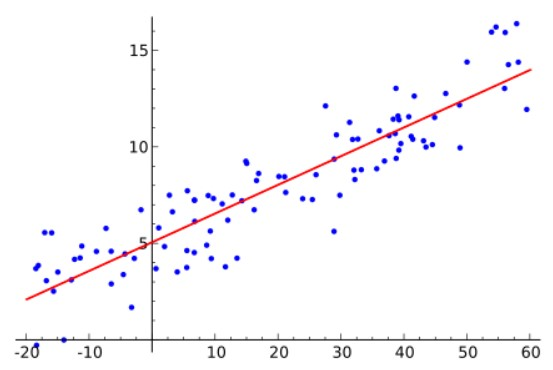
\includegraphics[width=0.75\linewidth]{2/figures/regresion.jpg}
			\caption{Regresión}
		\end{subfigure}%
		\begin{subfigure}{.5\textwidth}
			\centering
			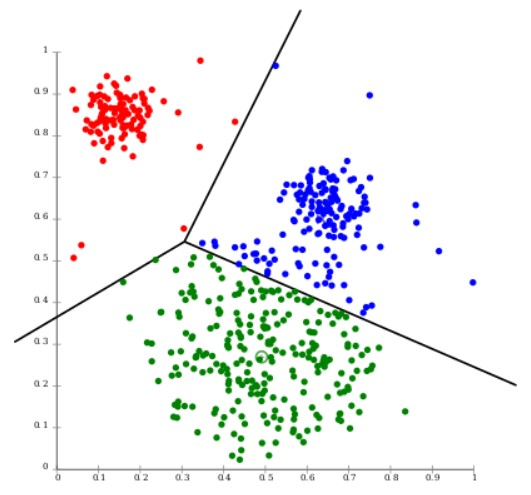
\includegraphics[width=0.65\linewidth]{2/figures/clasificacion.jpg}
			\caption{Clasificación}
		\end{subfigure}
		\caption[Ejemplo de algoritmos de regresión y clasificación]{Ejemplo de algoritmos de regresión y clasificación. Fuente: \cite{bk_zambrano2018supnosup}}
		\label{2:fig1}
	\end{figure}
	
	Para el segundo tipo de aprendizaje supervisado, el algoritmo más usado es el de los K Vecinos más cercanos o \textit{k-NN Nearest Neighbour} en inglés. Este se basa en la idea de que los nuevos ejemplos serán clasificados a la clase a la cual pertenezca la mayor cantidad de vecinos más cercanos del conjunto de entrenamiento más cercano a él. Sin embargo, el número k de vecinos más cercanos lo decide el usuario, de preferencia impar, para evitar ambigüedad al momento de clasificar un registro por parte del algoritmo (esto puede ocasionarse por las mismas distancias existentes entre dos o más registros). Otra variante aplicada consiste en la ponderación de cada vecino de acuerdo a la distancia entre él y el ejemplar a ser clasificado, asignando mayor peso a los más próximos \parencite{tec_sancho2018supnosup}. Para ello, se tiene la Ecuación \ref{eq:weights-KNN} y su variante en la Ecuación \ref{eq:weights-KNN_alt}:	
	%\begin{equcaption}[!ht]
	\begin{equation}\label{eq:weights-KNN}
	\phantomsection
	W_i = \frac{1}{d(x, x_i)^2}
	\end{equation}
	\myequations{Cálculo de los pesos para el algoritmo K-NN mediante ponderación de sus distancias}
	%\caption[Cálculo de los pesos para el algoritmo K-NN mediante ponderación de sus distancias]{Cálculo de los pesos para el algoritmo K-NN mediante ponderación de sus distancias. Fuente: \cite{tec_sancho2018supnosup}}
	%\end{equcaption}

	%\begin{equcaption}[!ht]
	\begin{equation}\label{eq:weights-KNN_alt}
	\phantomsection
	argmax_{v \in V}\sum_{i=1…k,x_i \in v}W_i
	\end{equation}
	\myequations{Fórmula alternativa del algoritmo K-NN mediante sumatoria de pesos}
	%\caption[Fórmula alternativa del algoritmo K-NN mediante sumatoria de pesos]{Fórmula alternativa del algoritmo K-NN mediante sumatoria de pesos. Fuente: \cite{tec_sancho2018supnosup}}
	%\end{equcaption}

	Donde:
	\begin{conditions}
		x	&	ejemplo que se desea clasificar \\
		V	&	posibles clases de clasificación \\
		x_i   &  conjunto de los k ejemplos de entrenamiento más cercanos
	\end{conditions}
		
	y finalmente, la clase asignada a $x$ es aquella que verifique que la suma de los pesos de sus representantes sea la máxima, representándose en la Figura \ref{2:fig2}:
	
	\begin{figure}[h]
		\begin{center}
			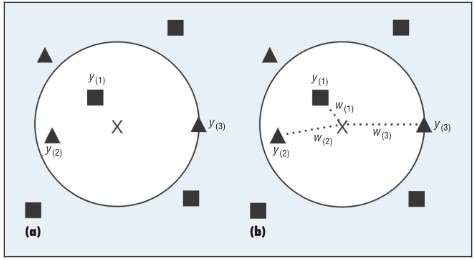
\includegraphics[width=0.55\textwidth]{2/figures/knn.jpg}
			\caption[Algoritmo de K Vecinos más cercanos con pesos ponderados]{Algoritmo de K Vecinos más cercanos con pesos ponderados. Fuente: \cite{tec_sancho2018supnosup}}
			\label{2:fig2}
		\end{center}
	\end{figure}
	
	\item \textbf{Aprendizaje no supervisado}: A diferencia de la anterior, aquí se trabaja con datos no etiquetados para entrenar el modelo, ya que el fin es de carácter exploratorio y descriptivo de la estructura de los datos. No existen variables independientes o Y.
	
	La función es agrupar ejemplares, por lo que el algoritmo los cataloga por similitud en sus características y a partir de ahí, crea grupos o clústeres sin tener la capacidad de definir cómo es cada individualidad de cada uno de los integrantes de los mismos \parencite{bk_zambrano2018supnosup}.
	
	El algoritmo usado para este tipo de aprendizaje es el de las K medias o \textit{k-means} en inglés. Este intenta encontrar una partición de las muestras en K agrupaciones, de manera que cada ejemplar pertenezca a una de ellas de acuerdo al centroide más cercano. Si bien el valor de K es definido por el usuario, a partir de pruebas de varias iteraciones se le puede consultar al algoritmo cuál es su valor óptimo. La función para lograr esto se observa en la Ecuación \ref{eq:k-means}:
	%\begin{equcaption}[!ht]
	\begin{equation}\label{eq:k-means}
	\phantomsection
	\sum_{i}\sum_{j}\mathrm{d}(x_j^i, c_i)^2
	\end{equation}
	\myequations{Fórmula del algoritmo k-means}
	%\caption[Fórmula del algoritmo k-means]{Fórmula del algoritmo k-means. Fuente: \cite{tec_sancho2018supnosup}}
	%\end{equcaption}
	
	Donde:
	\begin{conditions}
		c_i   &  centroide de la agrupación i-ésima \\
		x_j^i   &  conjunto de ejemplos clasificados de la agrupación i-ésima
	\end{conditions}
	
	Representándose en la Figura \ref{2:fig3}, los pasos seguidos para este algoritmo comienzan con la selección de los K puntos como como centros de los grupos. Luego, se asignarán los ejemplos al centro más cercano y se calculará el centroide de los ejemplos asociados a cada grupo. Finalmente, estos dos últimos pasos se repetirán hasta que ninguno de los centros pueda ser reasignados en las iteraciones.
	\begin{figure}[h]
		\begin{center}
			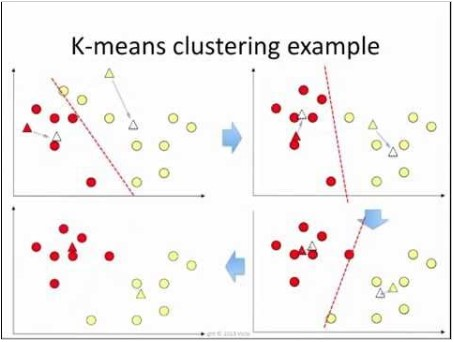
\includegraphics[width=0.50\textwidth]{2/figures/kmeans.jpg}
			\caption[Funcionamiento del algoritmo de K medias]{Funcionamiento del algoritmo de K medias. Fuente: \cite{tec_sancho2018supnosup}}
			\label{2:fig3}
		\end{center}
	\end{figure}
		
	\item \textbf{Aprendizaje por refuerzo}: Se basa en que un agente racional puede tomar una decisión a partir de una retroalimentación llamada recompensa o refuerzo. A diferencia del Aprendizaje Supervisado, en donde el agente puede aprender solamente a partir de ejemplos dados, en este caso no basta solamente con proporcionárselos sino también de “informarle” si lo está haciendo de la manera correcta o no. Por ejemplo, un agente que intenta aprender a jugar ajedrez necesita saber que algo bueno ha ocurrido cuando gana y algo malo ha ocurrido cuando pierde. La mejor recompensa que busca al finalizar el juego es vencer al oponente, y para ello debe estudiar todos los movimientos que este haga, la posición de las fichas en el tablero, entre otros. A este conjunto se le conoce como entorno o medio ambiente \parencite{bk_russell2004intart}. Entonces, en resumen, representando en la Figura \ref{2:fig4}, y mencionando otro ejemplo, el aprendizaje por refuerzo está compuesto por un agente (Pacman) en un estado determinado (su ubicación o posición actual) dentro de un medio ambiente (el laberinto). La recompensa positiva que busca Pacman son los puntos por comer, mientras que la negativa será la de morir si se cruza con un fantasma, en base a la acción (desplazamiento a un nuevo estado) que realice \parencite{tec_merino2019aprendrefuerzo}.
	\begin{figure}[h]
		\begin{center}
			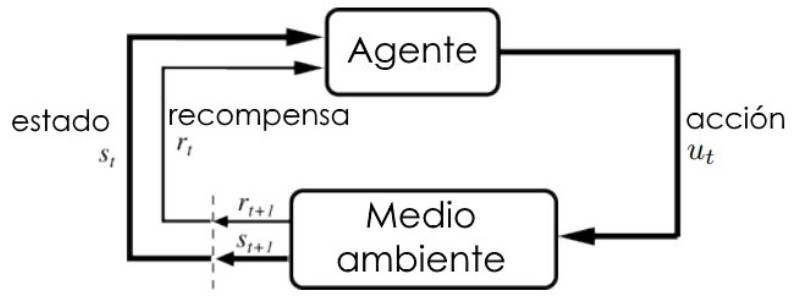
\includegraphics[width=0.60\textwidth]{2/figures/aprendizaje_refuerzo.jpg}
			\caption[Componentes del Aprendizaje por Refuerzo]{Componentes del Aprendizaje por Refuerzo. Fuente: \cite{bk_sutton2018rl}}
			\label{2:fig4}
		\end{center}
	\end{figure}
\end{itemize}

\clearpage

\subsection{Aprendizaje Profundo}

El Aprendizaje Profundo (\textit{Deep Learning} por su nombre en inglés) es un tipo de Aprendizaje Automático que entrena a una computadora para que realice tareas como las realizadas por los seres humanos, desde la identificación de imágenes hasta realizar predicciones y reconocer el lenguaje humano. El Aprendizaje Profundo configura parámetros básicos acerca de los datos y entrena a la computadora para que aprenda por su cuenta reconociendo patrones mediante el uso de múltiples capas de procesamiento \parencite{gl_sas_deeplearning}. Se basa en teorías acerca de cómo funciona el cerebro humano \parencite{tec_banafa2019deeplearning}.

La principal diferencia con el Aprendizaje Automático es que el Aprendizaje Profundo se basa en la extracción de características y clasificación al mismo tiempo luego de recibir una entrada, algo que en la primera técnica ocurre por separado, como se aprecia en la Figura \ref{2:fig5}.
\begin{figure}[!ht]
	\begin{center}
		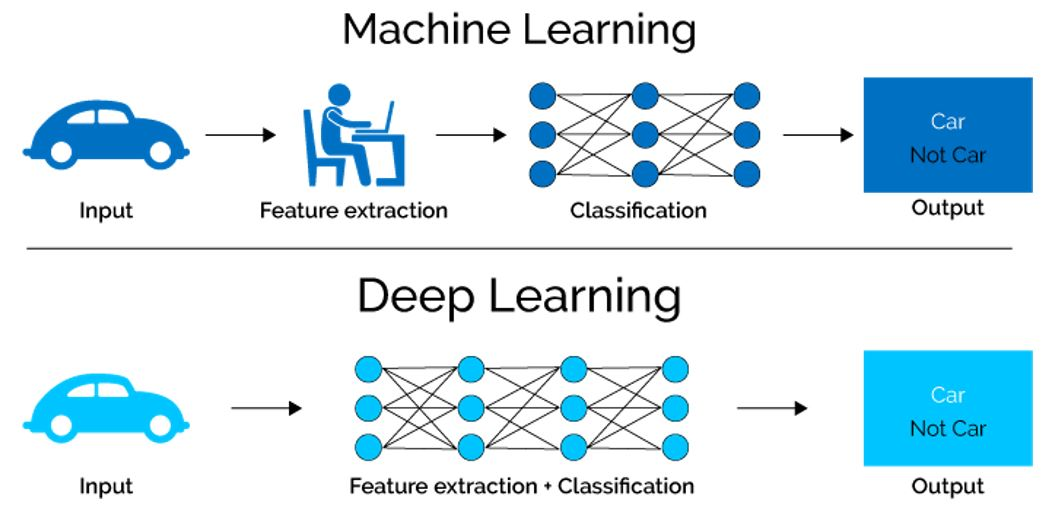
\includegraphics[width=0.70\textwidth]{2/figures/deeplearning_machinelearning.jpg}
		\caption[Diferencia entre Aprendizaje Automático y Aprendizaje Profundo]{Diferencia entre Aprendizaje Automático y Aprendizaje Profundo. Fuente: \cite{tec_cook2018deeplearning}}
		\label{2:fig5}
	\end{center}
\end{figure}

Por un lado, mientras en el Aprendizaje Automático o de máquina, el ordenador extrae conocimiento a través de experiencia supervisada, en el aprendizaje profundo está menos sometido a supervisión. Mientras que el primer tipo de aprendizaje consume muchísimo tiempo y se basa en proponer abstracciones que permiten aprender al ordenador, en el segundo no consume demasiado tiempo y por el contrario de su par, crea redes neuronales a gran escala que permiten que el ordenador aprenda y piense por sí mismo sin necesidad directa de intervención humana. Actualmente, el Aprendizaje Profundo se usa para crear softwares capaces de determinar emociones o eventos descritos en textos, reconocimiento de objetos en fotografías y realizar predicciones acerca del posible comportamiento futuro de las personas. Empresas como Google (proyecto Google Brain) o Facebook (Unidad de investigación en IA) han puesto en marcha proyectos basados en esta rama para potenciar y mejorar sus algoritmos con el fin de ofrecer una mejor experiencia de sus servicios a sus clientes \parencite{tec_banafa2019deeplearning}.

\subsection{Modelo Predictivo}

Son modelos de datos estadísticos utilizados para predecir el comportamiento futuro. En estos, se recopilan datos históricos y actuales, se formula un modelo estadístico, se realizan predicciones y el modelo se valida a medida que se dispone de datos adicionales. Los modelos predictivos analizan el rendimiento pasado para evaluar la probabilidad de que un cliente muestre un comportamiento específico en el futuro. En esta categoría también abarca la búsqueda de patrones ocultos \parencite{gl_gartner2019pm}.

\subsection{Minería de Datos}

La Minería de Datos es un campo de la estadística y las ciencias de la computación referido al proceso que intenta descubrir patrones en grandes volúmenes de conjuntos de datos \parencite{bk_maimon2010datamining}. Normalmente, estos patrones no pueden detectarse mediante la exploración tradicional de datos porque sus relaciones son demasiado complejas o por su gran volumen. Para ello, utiliza métodos de Inteligencia Artificial, Aprendizaje Automático, estadística y sistemas de bases de datos. Estos patrones son recopilados y definidos como un modelo de minería de datos, los cuales pueden aplicarse en los siguientes escenarios \parencite{gl_microsoft2019datamining}:
\begin{itemize}
	\item Previsión.
	\item Riesgo y probabilidad.
	\item Recomendaciones.
	\item Buscar secuencias.
	\item Agrupación.
\end{itemize}

La generación de un modelo de minería de datos forma de un macro-proceso descrita en los siguientes seis pasos representados en la Figura \ref{2:fig6} \parencite{gl_microsoft2019datamining}:
\begin{figure}[h]
	\begin{center}
		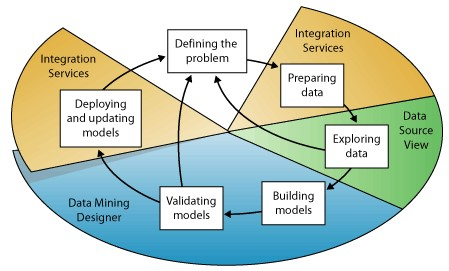
\includegraphics[width=0.7\textwidth]{2/figures/data_mining_steps.jpg}
		\caption[Diagrama de los seis pasos básicos]{Diagrama de los seis pasos básicos. Fuente: \cite{gl_microsoft2019datamining}}
		\label{2:fig6}
	\end{center}
\end{figure}

\clearpage

\subsection{Metodologías de Minería de Datos}

Dentro de los sistemas de analítica de negocio, Big Data y Minería de Datos, las tres metodologías más usadas se encuentran CRISP-DM, SEMMA y KDD \parencite{tec_braulio2015metodologiasdm}.
\begin{itemize}
	\item \textbf{CRISP-DM} (Cross Industry Standard Process for Data Mining):
	
	Esta metodología presenta seis fases representadas en la Figura \ref{2:fig7} a continuación.
	\begin{figure}[h]
		\begin{center}
			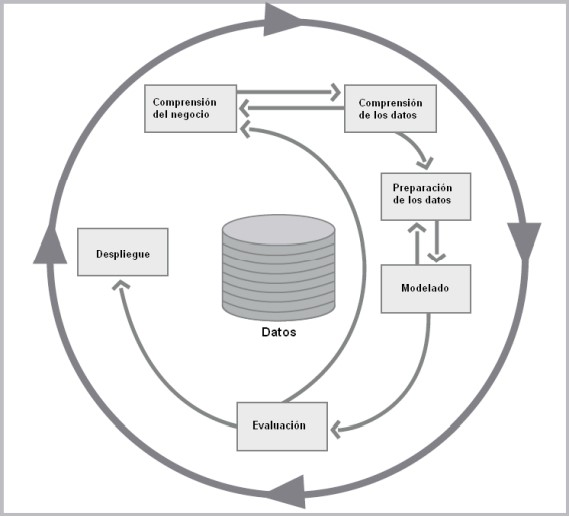
\includegraphics[width=0.65\textwidth]{2/figures/crispdm.jpg}
			\caption[Fases de la metodología CRISP-DM]{Fases de la metodología CRISP-DM. Fuente: \cite{tec_braulio2015metodologiasdm}}
			\label{2:fig7}
		\end{center}
	\end{figure}
		
	\begin{itemize}
		\item En la comprensión del negocio se determinan los objetivos y requerimientos desde el lado del negocio, así como generar plan del proyecto.
		\item En la comprensión de los datos se logra entender el significado de las variables existentes, así como el entendimiento de los datos desde su recopilación hasta su verificación de calidad.
		\item En la preparación de los datos se prepara el conjunto de datos adecuado que servirán para la construcción del modelo. Por ello, la calidad de los datos es un factor relevante y ello requiere la exclusión de redundancia y valores que no ayuden a establecer buena comprensión y resultados más adelante. A esto se le conoce como limpieza de datos.
		\item En el modelado se aplican técnicas de minería de datos en el conjunto de datos creado en el paso anterior. Para ello, se evalúan entre varias la que mejor performance desempeñe y luego se construye el o los modelos que busquen determinar un objetivo.
		\item En la evaluación se evalúan los posibles modelos del paso anterior a partir del nivel de importancia de acuerdo a las necesidades del negocio y performance que estos cuentan.
		\item El despliegue, finalmente, utiliza el modelo final creado para determinar los objetivos que se buscan cumplir en los requerimientos y ayudar en la toma de decisiones.
	\end{itemize}
	
	\item \textbf{SEMMA} (Sample – Explore – Modify – Model – Assess):
	
	Esta metodología cuenta con cinco fases como se aprecia en la Figura \ref{2:fig8}. A diferencia de la anterior, esta metodología se enfoca más en el modelado.
	\begin{figure}[h]
		\begin{center}
			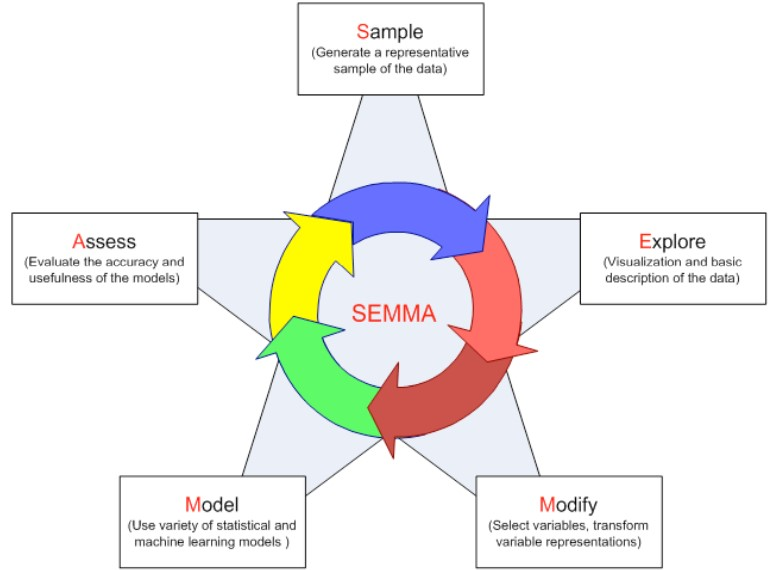
\includegraphics[width=0.70\textwidth]{2/figures/semma.jpg}
			\caption[Fases de la metodología SEMMA]{Fases de la metodología SEMMA. Fuente: \cite{tec_braulio2015metodologiasdm}}
			\label{2:fig8}
		\end{center}
	\end{figure}
	
	\begin{itemize}
		\item En la Muestra (\textit{Sample}) se crea una muestra significativa.
		\item En la Exploración (\textit{Explore}) se comprenden los datos con el fin de encontrar relaciones entre variables y anomalías.
		\item En la Modificación (\textit{Modify}) se transforman las variables para las necesidades del modelo.
		\item En la Modelización (\textit{Model}) se aplican uno o varios modelos sobre el conjunto de datos para buscar resultados.
		\item En el Asesoramiento (\textit{Assessment}) se evalúan los resultados obtenidos del modelo.
	\end{itemize}
	
	\item \textbf{KDD} (Knowledge Discovery and Data Mining):
	
	Esta metodología se refiere al proceso de encontrar conocimiento alguno en el dato y, a diferencia de sus predecesores, se enfoca en crear aplicaciones de minería de datos. Consta de cinco fases más 1 previa y 1 posterior basadas en la generación de conocimiento como se muestra en la Figura \ref{2:fig9}.
	\begin{figure}[h]
		\begin{center}
			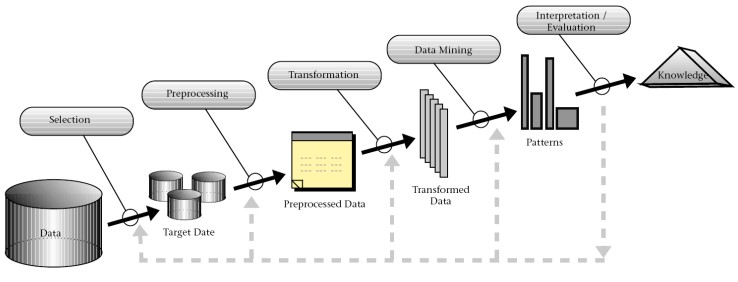
\includegraphics[width=0.80\textwidth]{2/figures/kdd.jpg}
			\caption[Fases de la metodología KDD]{Fases de la metodología KDD. Fuente: \cite{tec_braulio2015metodologiasdm}}
			\label{2:fig9}
		\end{center}
	\end{figure}
	
	\begin{itemize}
		\item En la fase Pre KDD se comprende el dominio del negocio, así como también se identifican las necesidades del cliente.
		\item En la selección, primero se identifica el conjunto de datos a usar y luego se seleccionan la muestra y las variables para la exploración.
		\item En el pre-procesamiento, se realiza la limpieza de datos y se elimina el ruido, así como los valores atípicos.
		\item En la transformación se implementan métodos de reducción de dimensiones para reducir el número de variables efectivas.
		\item En la Minería de datos, se elige el tipo de tarea de minería de datos (clasificación, regresión, agrupamiento, entre otros) así como el algoritmo, los métodos, los modelos y parámetros apropiados.
		\item En la interpretación y evaluación se analizan los resultados dados.
		\item En la fase Post KDD finalmente se consolida el conocimiento adquirido.
	\end{itemize}

\end{itemize}

Luego de presentar las tres metodologías más usadas, la pregunta dada es ¿cuál de los tres representa la mejor opción para usar?
Las tres metodologías tienen distinto número de pasos, así como distintos enfoques, tal cual se observa en el siguiente resumen de la Tabla \ref{2:table1}.

\begin{table}[htbp]
	\newcommand{\multirot}[1]{\multirow{2}{*}[-8ex]{\rotcell{\rlap{#1}}}}
	%\scriptsize
	\footnotesize
	\centering
	\begin{tabular}{|M{3cm}|M{5cm}|M{3.5cm}|M{3.5cm}|}
		\hline
		\rowcolor[rgb]{0,0.251,0.502}
		\multicolumn{1}{|p{3cm}|}{\centering \textcolor{white}{Modelo de Procesos de Minería de Datos}} &
		\multicolumn{1}{|p{5cm}|}{\centering \textcolor{white}{KDD}} &
		\multicolumn{1}{|p{3.5cm}|}{\centering \textcolor{white}{CRISP-DM}} & 
		\multicolumn{1}{|p{3.5cm}|}{\centering \textcolor{white}{SEMMA}}
		\\
		\hline
		{Número de pasos}
		&9
		&6
		&5                                                        
		\\
		\hline
		{\multirow{9}{*}[-11ex]{Nombre de los pasos}}
		&Desarrollo y entendimiento de la aplicación
		&Entendimiento del negocio
		&- \\
		\cline{2-4}
		&Creación de un conjunto de datos de destino
		&\multirow{2}{*}[-2ex]{Entendimiento de los datos}
		&Muestreo
		\\
		\cline{2-2}\cline{4-4}
		&Limpieza de datos y pre-procesamiento
		&\multicolumn{1}{c|}{}
		&Exploración
		\\
		\cline{2-4}
		&Transformación de datos
		&Preparación de los datos
		&Modificación
		\\
		\cline{2-4}
		&Elección de la tarea adecuada de Minería de datos
		&\multirow{3}{*}[-3ex]{Modelamiento}
		&\multirow{3}{*}[-3ex]{Modelo}
		\\
		\cline{2-2}
		&Elección del algoritmo adecuado de Minería de datos
		&\multicolumn{1}{c|}{}
		&\multicolumn{1}{c|}{}
		\\
		\cline{2-2}
		&Implementación del algoritmo de Minería de datos
		&\multicolumn{1}{c|}{}
		&\multicolumn{1}{c|}{}
		\\
		\cline{2-4}
		&Interpretación de patrones minados
		&Evaluación
		&Evaluación
		\\
		\cline{2-4}          & Uso de conocimiento descubierto & Despliegue & -
		\\
		\hline
	\end{tabular}%
	\caption[Cuadro comparativo entre características de las tres metodologías]{Cuadro comparativo entre características de las tres metodologías. Fuente: \cite{tec_shafique2014dmmodels}}
	\label{2:table1}
\end{table}

Sin embargo, la elección depende de los involucrados que finalmente usarán el modelo en el negocio. La mayoría de investigadores siguen la metodología KDD debido a que es más completo y su exactitud. Para aquellos objetivos enfocados más en la compañía como la integración usada por SAS Enterprise Miner con su software se utilizan SEMMA y CRISP-DM. Esta última resulta ser más completa de acuerdo a los estudios.

\clearpage

\subsection{Técnicas de Minería de Datos}

Existe una gran variedad de técnicas para la Minería de Datos. Las más importantes y utilizadas en los antecedentes de la investigación se mencionan a continuación \parencite{gl_microsoft2018datamining}.

\begin{itemize}
	\item \textbf{Redes Neuronales Artificiales} (RNA): Es un sistema de computación que consiste en un número de elementos o nodos simples, pero altamente interconectados, llamados “neuronas”, que se organizan en capas que procesan información utilizando respuestas de estado dinámico a entradas externas \parencite{tec_inzaugarat2018ann}.
	
	Este sistema de programas y estructura de datos se aproxima al funcionamiento del cerebro humano. Una red neuronal implica tener un gran número de procesadores funcionando en paralelo, teniendo cada uno de ellos su propia esfera de conocimiento y acceso a datos en su memoria local. Normalmente, una se alimenta con grandes cantidades de datos y un conjunto dado de reglas acerca de las relaciones. Luego, un programa puede indicar a la red cómo debe comportarse en respuesta a un estímulo externo o si puede iniciar la actividad por sí misma \parencite{tec_banafa2019deeplearning}.
	
	Para entender mejor cómo funciona una red neuronal, hay que describir qué es una neurona. Una neurona es una célula del cerebro cuya función principal es la recogida, procesamiento y emisión de señales eléctricas. Debido a que se piensa que la capacidad de procesamiento de información del cerebro proviene de redes de este tipo de neuronas, los primeros trabajos en Inteligencia Artificial se basaron en crear redes neuronales artificiales para emular este comportamiento, en 1943 con un modelo matemático, mostrado en la Figura \ref{2:fig10}, por los ya mencionados anteriormente McCulloch y Pitts.
	\begin{figure}[h]
		\begin{center}
			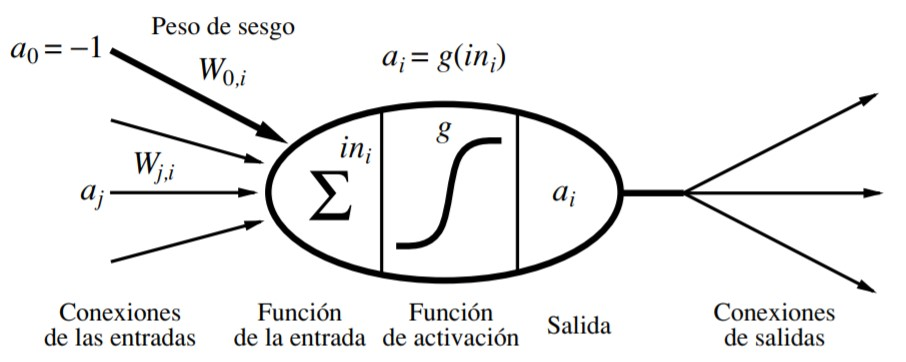
\includegraphics[width=0.75\textwidth]{2/figures/rnn_mcculloch.jpg}
			\caption[Modelo para representar una neurona propuesto por McCulloch y Pitts (1943)]{Modelo para representar una neurona propuesto por McCulloch y Pitts (1943). Fuente: \cite{bk_russell2004intart}}
			\label{2:fig10}
		\end{center}
	\end{figure}

	Estos y posteriores trabajos potenciaron lo que hoy en día se conoce como el campo de la neurociencia computacional \parencite{bk_russell2004intart}. Años más tarde, en 1958, se desarrolló el concepto del perceptrón por Rosenblatt, el cual tenía la capacidad de aprender y reconocer patrones sencillos, formado por entradas, neurona, función de adaptación (sigmoidal, tangencial, en escalón, etc.) y salida.
		
	La última figura descrita muestra, además de los pesos, funciones de activación tanto para la entrada ($a_j$) como para la salida ($a_i$). Pero, ¿qué son estas funciones y para qué sirven?
	
	Para comenzar, las redes neuronales están compuestas de nodos (la elipse) conectados a través de conexiones dirigidas (las flechas). Una conexión del nodo $j$ a la unidad $i$ sirve para propagar la activación $a_j$ de $j$ a $i$. Asimismo, cada conexión tiene un peso numérico $W(j,i)$ que determina la fuerza y el signo de la conexión. Para calcular cada nodo $i$, se realiza una suma ponderada de sus entradas (producto entre pesos y nodos de entrada $j$), y se le añade el sesgo (\textit{bias}) $\theta_i$ (aumenta/disminuye el valor de la combinación lineal de las entradas) como se observa en la Ecuación \ref{eq:nodo}:
	%\begin{equcaption}[!ht]
	\begin{equation}\label{eq:nodo}
	\phantomsection
	in_i=\sum_{j=0}^n W_{j,i}*a_j + \theta_i
	\end{equation}
	\myequations{Fórmula del cálculo del valor de un nodo i}
	%\caption[Fórmula del cálculo del valor de un nodo i]{Fórmula del cálculo del valor de un nodo \textit{i}. Fuente: \cite{bk_russell2004intart}}
	%\end{equcaption}
	
	Posteriormente, se efectúa una función de activación g a esta suma para producir la salida de la Ecuación \ref{eq:activacion}:
	%\begin{equcaption}[!ht]
	\begin{equation}\label{eq:activacion}
	\phantomsection
	a_i = g(in_i) = g \left(\sum_{j=0}^n W_{j,i}*a_j + \theta_i\right)
	\end{equation}
	\myequations{Fórmula de una función de activación g para la salida del nodo}
	%\caption[Fórmula de una función de activación g para la salida del nodo]{Fórmula de una función de activación g para la salida del nodo. Fuente: \cite{bk_russell2004intart}}
	%\end{equcaption}
	
	\clearpage
	
	Entonces, aquí se explica los dos objetivos de una función de activación. En primer lugar, se desea que el nodo esté “activo” (cercano a +1) cuando las entradas correctas sean dadas, e “inactiva” (cercano a 0) cuando las entradas erróneas sean proporcionadas. En segundo lugar, la activación tiene que ser no lineal porque, de lo contrario, la red neuronal colapsaría en su totalidad con una función lineal sencilla (Figura \ref{2:fig11}).
	\begin{figure}[h]
		\begin{center}
			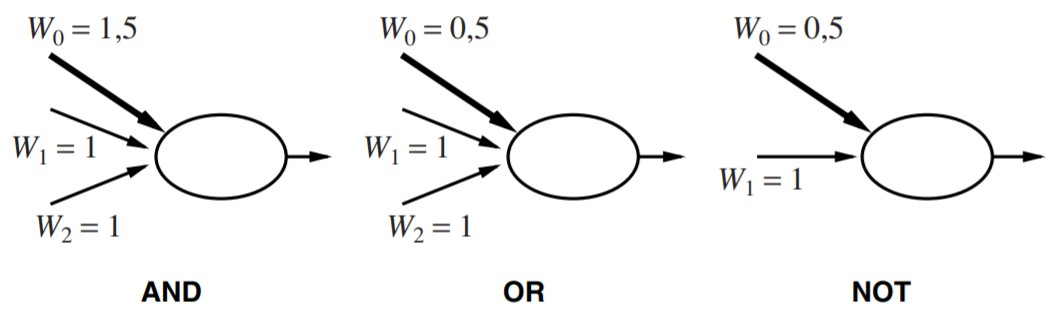
\includegraphics[width=0.75\textwidth]{2/figures/rna_activaciones.jpg}
			\caption[Nodos con funciones de activación umbral en forma de puertas lógicas]{Nodos con funciones de activación umbral en forma de puertas lógicas. Fuente: \cite{bk_russell2004intart}}
			\label{2:fig11}
		\end{center}
	\end{figure}
	
	Entre las funciones de activación que más destacan son las siguientes:
	\begin{itemize}
		\item \textbf{Función sigmoide o logística}: Toma los valores de entrada que oscilan entre infinito negativo y positivo, y restringe los valores de salida al rango entre 0 y 1. Frecuentemente es usada en Redes Multicapa (MLP) entrenadas con el algoritmo de propagación inversa. Se representa como en la Figura \ref{2:fig12} y su fórmula para calcular su nuevo valor es la Ecuación \ref{eq:sigmoide}:
		%\begin{equcaption}[!ht]
		\begin{equation}\label{eq:sigmoide}
		\phantomsection
		a=Logsig(n)=\frac{1}{1+e^{-n}}
		\end{equation}
		\myequations{Fórmula de la función de activación sigmoide}
		%\caption[Fórmula de la función de activación sigmoide]{Fórmula de la función de activación sigmoide. Fuente: \cite{pr_dorofki2012ann}}
		%\end{equcaption}
		
		\begin{figure}[h]
			\begin{center}
				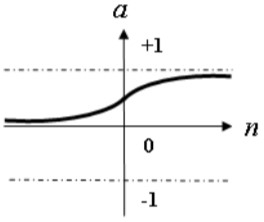
\includegraphics[width=0.3\textwidth]{2/figures/sigmoide.jpg}
				\caption[Función de activación sigmoide]{Función de activación sigmoide. Fuente: \cite{pr_dorofki2012ann}}
				\label{2:fig12}
			\end{center}
		\end{figure}
		
		Un dato curioso de esta función relacionado con la regresión logística es que el nombre de esta última no deriva de una regresión. Por el contrario, se debe a que, al principio de la neurona, se realiza una combinación lineal muy parecida a una regresión lineal y después se aplica la función logística o sigmoide. De ahí el origen del nombre \parencite{gl_iartificial2019reglogistica}.
		\begin{itemize}
			\item \textbf{Regresión Logística}: Como se mencionó antes, es similar a un modelo de regresión lineal, pero está adaptado para modelos en los que la variable dependiente es dicotómica, es decir, presenta solo dos posibles valores. Resulta muy útil para los casos en los que se desea predecir la presencia o ausencia de una característica o resultado según los valores de un conjunto de predictores \parencite{gl_ibm2019reglogistica}. Su función de coste que se optimiza con gradiente descendiente se representa mediante la Ecuación \ref{eq:logistica}:
			%\begin{equcaption}[!ht]
			\begin{equation}\label{eq:logistica}
			\phantomsection
			J(\theta)=\frac{1}{m}\sum_{i=1}^m [-y_i*\log(h_{\theta}(x_{i}))-(1-y_i)*\log(1-h_{\theta}(x_{i}))]
			\end{equation}
			\myequations{Fórmula de función de coste de una regresión logística}
			%\caption[Fórmula de función de coste de una regresión logística]{Fórmula de función de coste de una regresión logística. Fuente: \cite{gl_pardo_reglogcosto}}
			%\end{equcaption}
			
			Donde:
			\begin{conditions}
				h_{\theta}(x_{i})	&	función sigmoide de $\theta^T x$ \\
				\theta	&	vector de longitud theta para j=0,1,2,3...n \\
				x   &  matriz de entradas \\
				y	&  vector de salidas
			\end{conditions}
			
			La primera parte de la ecuación está conformada por el logaritmo de la probabilidad de éxito y la segunda, por la de fracaso.
			
			\item \textbf{Gradiente descendiente}: Es un método de optimización numérica para estimar los mejores coeficientes, fundamental en Deep Learning para entrenar redes neuronales y en muchos casos, para la regresión logística. A través de una función E(W), proporciona el error que comete la red en función del conjunto de pesos sinápticos W. El objetivo del aprendizaje será encontrar la configuración de pesos que corresponda al mínimo global de la función de error o coste \parencite{tec_bertona2005algevol}.
			
			En general, la función de error es una función no lineal, por lo que el algoritmo realiza una búsqueda a través del espacio de parámetros que, se aproxime de forma iterada a un error mínimo de la red para los parámetros adecuados, como se aprecia en la Figura \ref{2:fig13} \parencite{tec_sancho2017descentgrad}.
			\begin{figure}[h]
				\begin{center}
					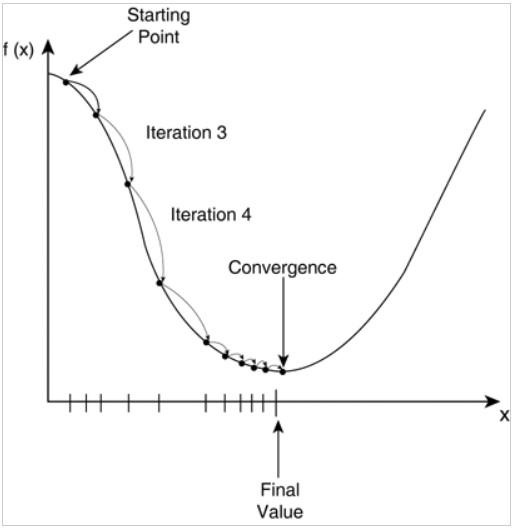
\includegraphics[width=0.35\textwidth]{2/figures/gradiente_descendiente.jpg}
					\caption[Ilustración del algoritmo gradiente descendiente]{Ilustración del algoritmo gradiente descendiente. Fuente: \cite{tec_sancho2017descentgrad}}
					\label{2:fig13}
				\end{center}
			\end{figure}
			
			El Descenso del Gradiente, como también se le conoce, es el algoritmo de entrenamiento más simple y también el más extendido y conocido. Solo hace uso del vector gradiente, y por ello se dice que es un método de primer orden \parencite{tec_sancho2017descentgrad}. Un gradiente es la generalización de la derivada. Matemática, la derivada de una función mide la rapidez con la que cambia el valor de esta, según varié el valor de su variable independiente. La gradiente se calcula con derivadas parciales, por lo que al actualizar los coeficientes W para un tiempo t, se usa la Ecuación \ref{eq:w_descgrad} \parencite{gl_iartificial2019descentgrad}:
			%\begin{equcaption}[!ht]
			\begin{equation}\label{eq:w_descgrad}
			\phantomsection
			W_{(t+1)}=W_{(t)}-\alpha \left(\frac{\partial MSE}{\partial W} \right)
			\end{equation}
			\myequations{Actualización de pesos W mediante gradiente descendiente}
			%\caption[Actualización de pesos W mediante gradiente descendiente]{Actualización de pesos W mediante gradiente descendiente. Fuente: \cite{gl_iartificial2019descentgrad}}
			%\end{equcaption}
		
			Donde: $\alpha$ = ratio de aprendizaje
			
			Este ratio controla el tamaño de la actualización. Si este es demasiado grande, será más difícil encontrar los coeficientes que minimicen la función de coste o error; la actualización de W es proporcional al gradiente; y se usa la resta para ir en dirección opuesta al gradiente como en la Figura \ref{2:fig14}.
			\begin{figure}[h]
				\begin{center}
					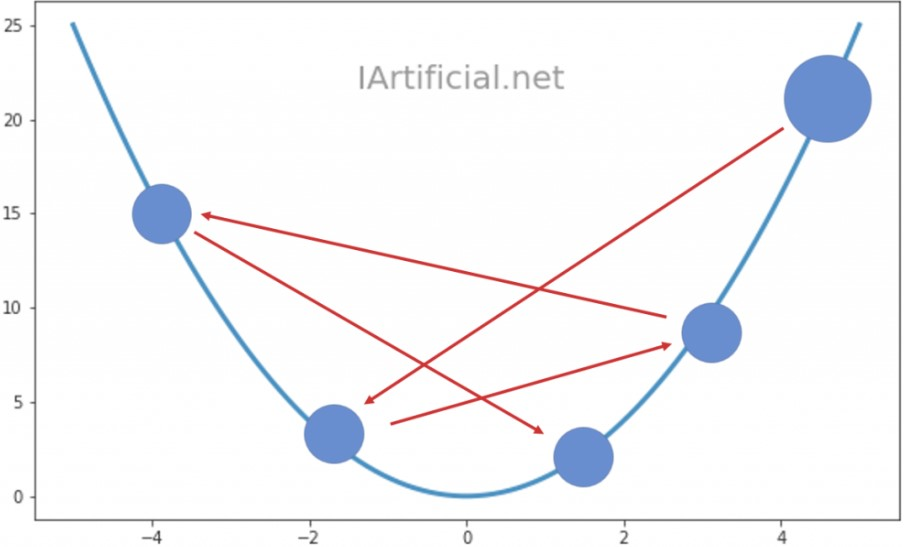
\includegraphics[width=0.45\textwidth]{2/figures/pesos_graddescen.jpg}
					\caption[Actualización de pesos W con el algoritmo]{Actualización de pesos W con el algoritmo. Fuente: \cite{gl_iartificial2019descentgrad}}
					\label{2:fig14}
				\end{center}
			\end{figure}
			
			\item \textbf{Propagación hacia atrás}: También conocido en inglés como \textit{Backpropagation}, es un método que consta de dos fases: en la primera se aplica un patrón, el cual se propaga por las distintas capas que componen la red hasta producir la salida de la misma. Luego, esta se compara con la salida deseada y se calcula el error cometido por cada neurona de salida. Estos errores se transmiten hacia atrás, partiendo de la capa de salida, hacia todas las neuronas de las capas intermedias [Fritsch, 1996] \parencite{tec_bertona2005algevol}. La actualización iterativa de los pesos que el algoritmo propone es mediante la Ecuación \ref{eq:backpropagation}:
			%\begin{equcaption}[!ht]
			\begin{equation}\label{eq:backpropagation}
			\phantomsection
			W_{ji}(t+1)=W_{ji}(t)+[\alpha \delta_{pj} y_{pj} + \beta \Delta W_{ji}(t)]
			\end{equation}
			\myequations{Fórmula del algoritmo de propagación hacia atrás}
			%\caption[Fórmula del algoritmo de propagación hacia atrás]{Fórmula del algoritmo de propagación hacia atrás. Fuente: \cite{tec_bertona2005algevol}}
			%\end{equcaption}
		
			\begin{equation}
			%\phantomsection
			\text{siendo} \quad \delta_{pj} =
			\left\{
			\begin{aligned}
				(d_{pj}-y_{pj})f'_j(h_j) \quad\text{si j es una neurona de salida}\\
				\left(\sum_{k} \delta_{pk} W_{kj}\right)f'_j(h_j) \quad\text{si j es una neurona oculta}
			\end{aligned}
			\right.
			\end{equation}
			\myequations{pendiente}
			
			\begin{figure}[h]
				\begin{center}
					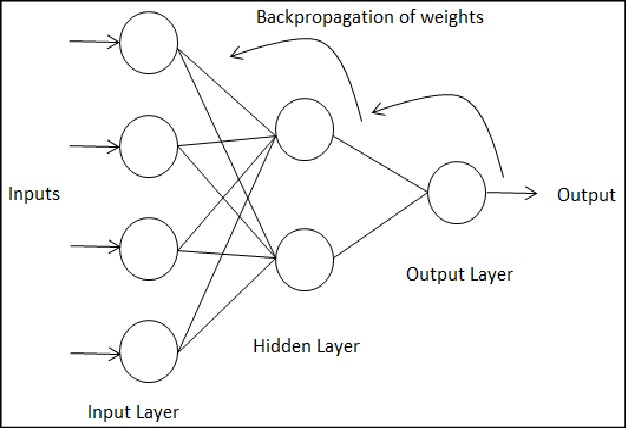
\includegraphics[width=0.5\textwidth]{2/figures/backpropagation.jpg}
					\caption[Capa oculta simple MLP con propagación hacia atrás]{Capa oculta simple MLP con propagación hacia atrás. Fuente: \cite{gl_iartificial2019descentgrad}}
					\label{2:fig15}
				\end{center}
			\end{figure}
			
			Para entender mejor la teoría y la fórmula de actualización de pesos, se seguirá el siguiente ejemplo del conjunto de redes de la Figura \ref{2:fig16}.
			
			\clearpage
			\begin{figure}[h]
				\begin{center}
					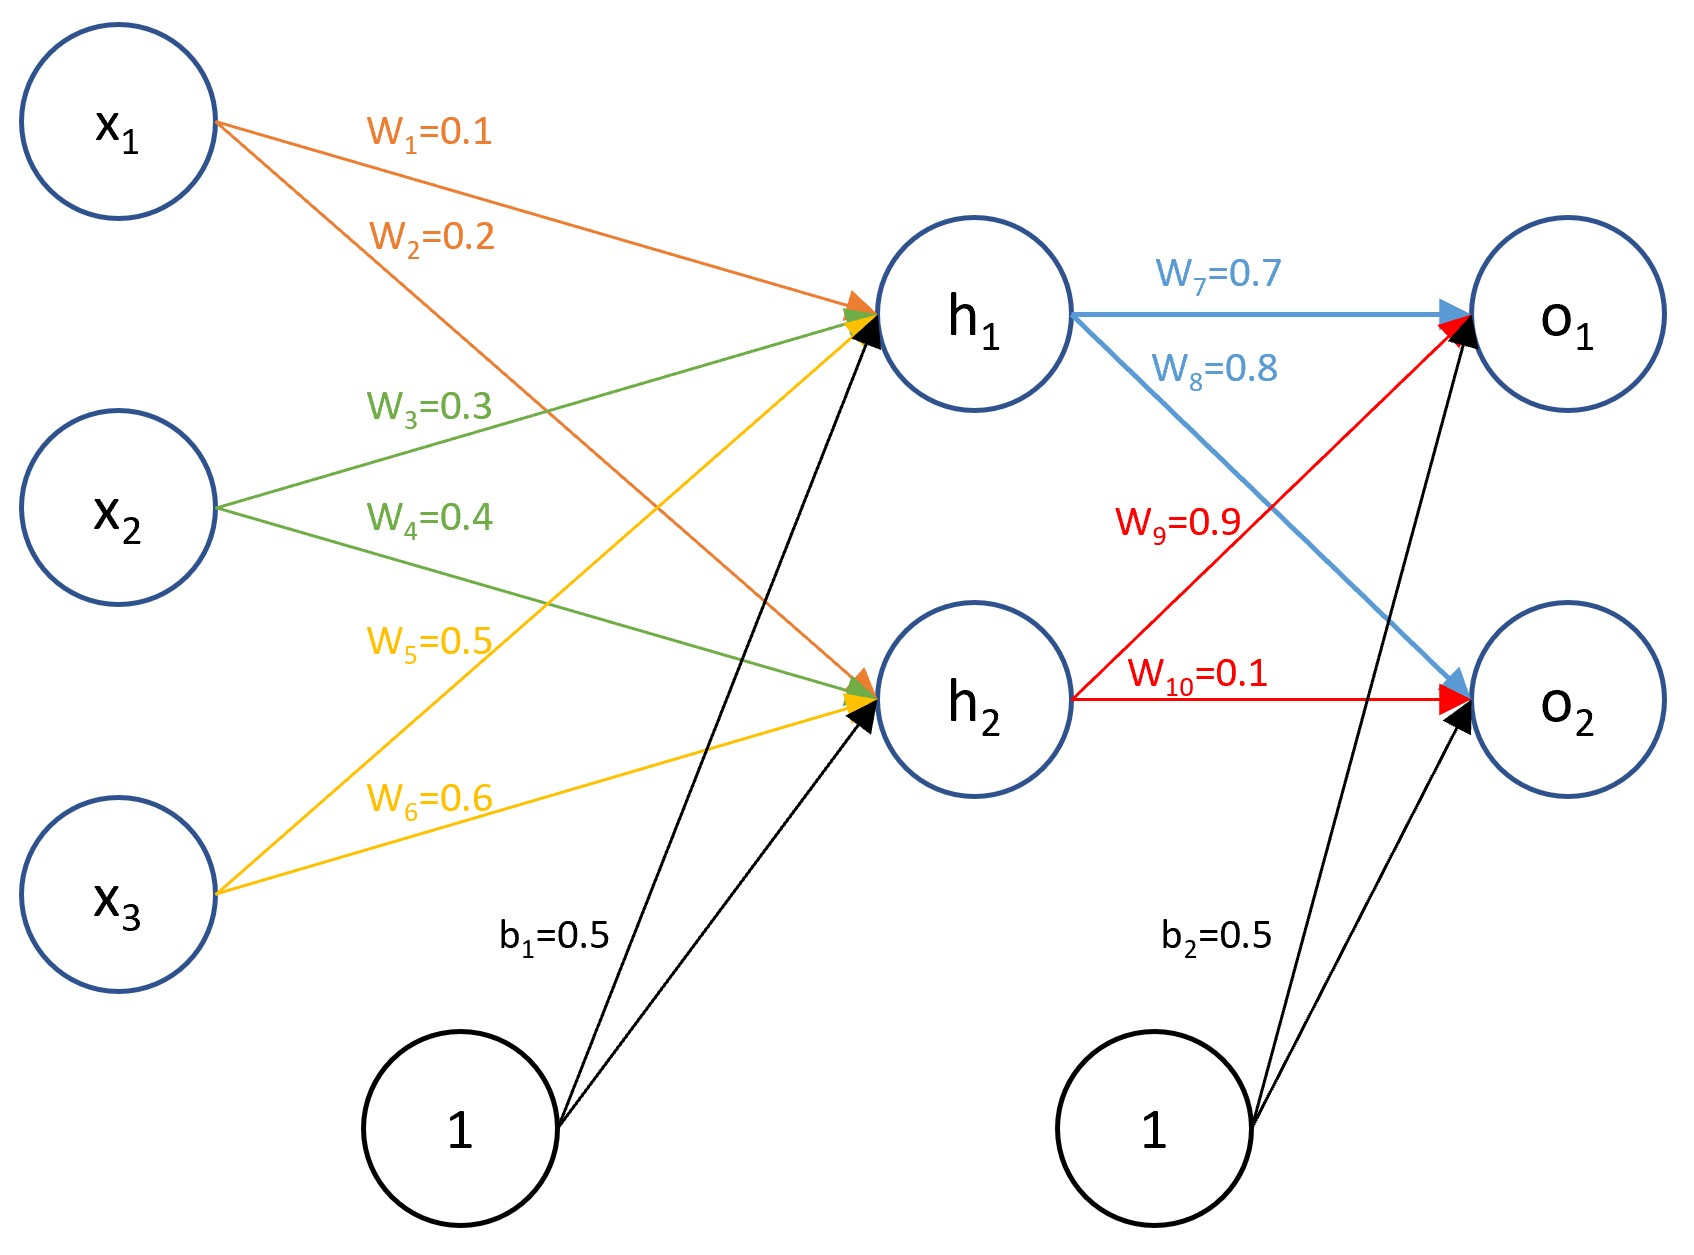
\includegraphics[width=0.55\textwidth]{2/figures/rna_pesos.jpg}
					\caption[Redes neuronales de ejemplo]{Redes neuronales de ejemplo. Fuente: \cite{gl_ansrw2019backpropagation}}
					\label{2:fig16}
				\end{center}
			\end{figure}
			
			Se tiene una red neuronal con tres nodos de entradas ($x_1$=1, $x_2$=4 y $x_3$=5) con dos pesos respectivos cada una ($W_1$=0.1 y $W_2$=0.2 para $x_1$; $W_3$=0.3 y $W_4$=0.4 para $x_2$; $W_5$=0.5 y $W_6$=0.6 para $x_3$), dos capas ocultas ($h_1$ y $h_2$) con dos peso cada una ($W_7$=0.7 y $W_8$=0.8 para $h_1$; $W_9$=0.9 y $W_10$=0.1 para $h_2$) y dos nodos de salida ($O_1$ y $O_2$).
			
			El proceso normal para calcular el valor del nodo final se da, tanto con los nodos de entrada y los de capa oculta, mediante la sumatoria de producto de cada peso con su valor, es decir, mediante la fórmula de las RNA $in_i=\sum_{j=0}^n W_{j,i}*a_j+b_{j,i}$, al mismo tiempo que devuelve un valor del error cometido. Este último se calcula mediante la Ecuación \ref{eq:rnaerror}:
			\begin{equcaption}[!ht]
				\begin{equation}
				\phantomsection
				E_k=(T_k-O_k)*O_k*(1-O_k)
				\end{equation}
				\caption[Cálculo del error cometido en una red neuronal]{Cálculo del error cometido en una red neuronal. Fuente: \cite{tec_viera2013backpropexplain}}
				\label{eq:rnaerror}
			\end{equcaption}
			
			Donde:
			\begin{conditions}
				T_k	&	salida correcta de cada nodo de salida \\
				O_k	&	salida actual que cada nodo genera
			\end{conditions}
			
			Con estos errores, se retrocede hacia la capa oculta y se procede a calcular los nuevos pesos para sus nodos. Esto se realiza mediante la Ecuación \ref{eq:updateweightsrna}:
			\begin{equcaption}[!ht]
				\begin{equation}
				\phantomsection
				W_{jk}=W_{jk}+L*E_k*O_j
				\end{equation}
				\caption[Actualización de pesos mediante propagación hacia atrás]{Actualización de pesos mediante propagación hacia atrás. Fuente: \cite{tec_viera2013backpropexplain}}
				\label{eq:updateweightsrna}
			\end{equcaption}
			
			Donde:
			\begin{conditions}
				W_{jk}	&	peso a actualizar para cada nodo de la capa oculta ($W_7$, $W_8$, $W_9$ y $W_{10}$) \\
				L	&	porcentaje de aprendizaje \\
				O_j	&	valor de los nodos que entrarán a las salidas
			\end{conditions}
			
			Estos nuevos pesos permitirán redefinir los errores de ambos nodos, con una pequeña diferencia en su cálculo (Ecuación \ref{eq:errornodorna}):
			\begin{equcaption}[!ht]
				\begin{equation}
				\phantomsection
				E_{j}=O_{j}*(1-O_{j})*\sum E_{k}*W_{jk}
				\end{equation}
				\caption[Cálculo de errores de nodos usando pesos actualizados]{Cálculo de errores de nodos usando pesos actualizados. Fuente: \cite{tec_viera2013backpropexplain}}
				\label{eq:errornodorna}
			\end{equcaption}
			
			El error de cada nodo de la capa oculta se obtiene multiplicando su valor por su complemento por la sumatoria del producto de sus pesos y los errores de los nodos de salida. Por ejemplo, para h1 sería 
			$E_{h1}=h_1*(1-h_1)*(0.7*O_1+0.8*O_2)$.
			
			Finalmente, se retrocede hacia los nodos de entrada y se repite el mismo proceso para la actualización de sus pesos y errores.
		\end{itemize}
	\item \textbf{Función tangente hiperbólica}: Esta función está relacionada con una sigmoide bipolar. Sin embargo, sus salidas estarán en el rango de -1 y +1. Para redes neuronales, donde la velocidad es más importante que la forma de la función misma, es recomendable usar esta. Se representa como en la Figura \ref{2:fig17} y su fórmula para calcular su nuevo valor es la Ecuación \ref{eq:tansig}:
	\begin{figure}[!ht]
		\begin{center}
			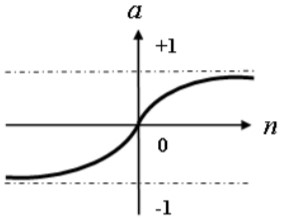
\includegraphics[width=0.30\textwidth]{2/figures/hiperbolica.jpg}
			\caption[Función de activación tangente hiperbólica]{Función de activación tangente hiperbólica. Fuente: \cite{pr_dorofki2012ann}}
			\label{2:fig17}
		\end{center}
	\end{figure}
	
	\begin{equcaption}[!ht]
		\begin{equation}
		\phantomsection
		a=Tansig(n)=\frac{2}{1+e^{-2n}}-1
		\end{equation}
		\caption[Fórmula de la función de activación tangente hiperbólica]{Fórmula de la función de activación tangente hiperbólica. Fuente: \cite{pr_dorofki2012ann}}
		\label{eq:tansig}
	\end{equcaption}

	\item \textbf{Función puramente lineal (purelin)}: Se caracteriza porque su salida es igual a su entrada debido a su linealidad. Normalmente se usa para obtener los mismos valores de entrada. Se representa en la Figura \ref{2:fig18} y se calcula mediante la Ecuación \ref{eq:purelin}:
	
	\begin{figure}[h]
		\begin{center}
			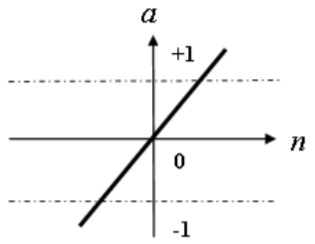
\includegraphics[width=0.30\textwidth]{2/figures/purelin.jpg}
			\caption[Función de activación puramente lineal]{Función de activación puramente lineal. Fuente: \cite{pr_dorofki2012ann}}
			\label{2:fig18}
		\end{center}
	\end{figure}

	\begin{equcaption}[!ht]
		\begin{equation}
		\phantomsection
		a=n
		\end{equation}
		\caption[Fórmula de la función de activación puramente lineal]{Fórmula de la función de activación puramente lineal. Fuente: \cite{pr_dorofki2012ann}}
		\label{eq:purelin}
	\end{equcaption}
	
	\item \textbf{Función Unidad Lineal Rectificada (ReLU)}: Se caracteriza por conservar los valores positivos y convertir los negativos de entrada en 0, con la finalidad de no considerarlos en la siguiente capa de convolución \parencite{gl_bigdata2019bigdata}. Si bien tiene un buen desempeño en redes convolucionales y es muy usada para procesar imágenes, al no estar acotada pueden morirse demasiadas neuronas \parencite{gl_calvo2018activrna}. Se representa en la Figura \ref{2:fig19} y se calcula mediante la Ecuación \ref{eq:relu}:
	\begin{figure}[h]
		\begin{center}
			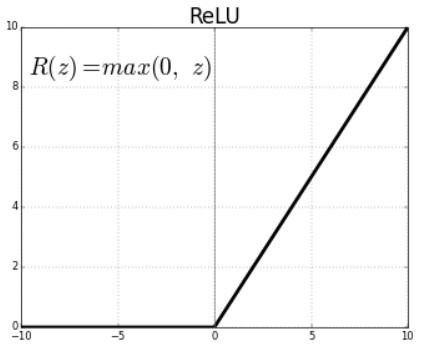
\includegraphics[width=0.30\textwidth]{2/figures/relu.jpg}
			\caption[Función de activación ReLU]{Función de activación ReLU. Fuente: \cite{gl_mlfa2019redesneuronales}}
			\label{2:fig19}
		\end{center}
	\end{figure}
	
	\begin{equcaption}[!ht]
		\begin{equation}
		\phantomsection
		f(x) = \max (0,x) =
		\left\{
		\begin{aligned}
		0 \quad \text{para} \quad x < 0\\
		x \quad \text{para} \quad x \geq 0
		\end{aligned}
		\right.
		\end{equation}
		\caption[Fórmula de la función de activación ReLU]{Fórmula de la función de activación ReLU. Fuente: \cite{gl_calvo2018activrna}}
		\label{eq:relu}
	\end{equcaption}
	
	\end{itemize}
	
	Además de existir distintas funciones de activación, las redes neuronales artificiales se clasifican según la topología de red, siendo algunas de las más importantes \parencite{gl_calvo2017clasifrna}.
	
	\begin{itemize}
		\item \textbf{Red Neuronal Monocapa – Perceptrón simple}: Es la red neuronal más simple ya que está compuesta solamente de una capa de neuronas que componen varios nodos de entrada para proyectar una capa de neuronas de salida, como se aprecia en la Figura \ref{2:fig20}. Esta última capa se calcula usando la misma Ecuación 4 que implica la suma de productos de cada uno de los pesos de los nodos de entrada con sus instancias, añadiéndole finalmente el sesgo, aquel que controla la predisposición de la neurona a disparar un 1 o 0 independientemente de los pesos, para que el valor resultante se le aplique la función de activación que ayudarán a modelar funciones curvas o no triviales \parencite{gl_mlfa2019redesneuronales}.
		\begin{figure}[h]
			\begin{center}
				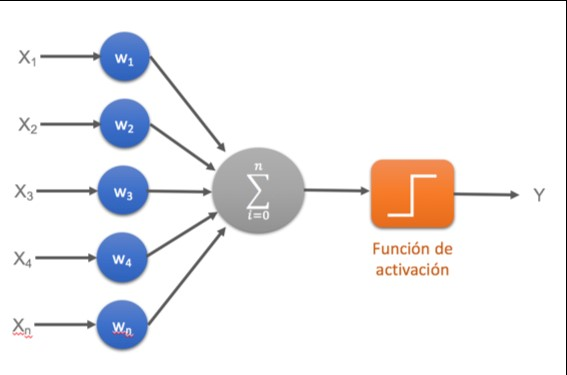
\includegraphics[width=0.45\textwidth]{2/figures/perceptron_simple.jpg}
				\caption[Ejemplo de perceptrón simple]{Ejemplo de perceptrón simple. Fuente: \cite{gl_calvo2017clasifrna}}
				\label{2:fig20}
			\end{center}
		\end{figure}
		
		\item \textbf{Red Neuronal Multicapa – Perceptrón multicapa}: Con arquitectura similar al perceptrón simple, con el añadido de contener capas intermedias entre la capa de neuronas de entrada y la de salida, conocidas como capas ocultas, como en el ejemplo de la Figura \ref{2:fig21}.
		\begin{figure}[h]
			\begin{center}
				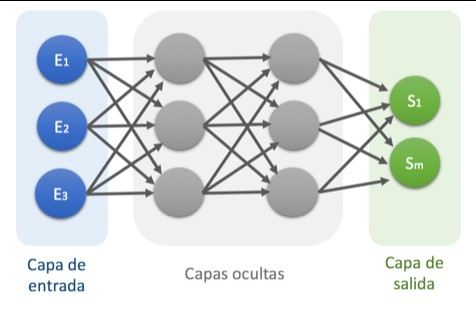
\includegraphics[width=0.50\textwidth]{2/figures/perceptron_multicapa.jpg}
				\caption[Ejemplo de perceptrón multicapa]{Ejemplo de perceptrón multicapa. Fuente: \cite{gl_calvo2017clasifrna}}
				\label{2:fig21}
			\end{center}
		\end{figure}
		
		\item \textbf{Redes Neuronales Convolucionales (CNN)}: También conocidas por su nombre en inglés \textit{Convolutional Neural Networks}, se diferencia del perceptrón multicapa en que cada neurona no necesita estar unida con todas las que le siguen, sino más bien solo con un subgrupo de estas con el fin de reducir la cantidad de neuronas necesarias para su funcionamiento, como se observa en la Figura \ref{2:fig22} \parencite{gl_calvo2017clasifrna}.
		\begin{figure}[h]
			\begin{center}
				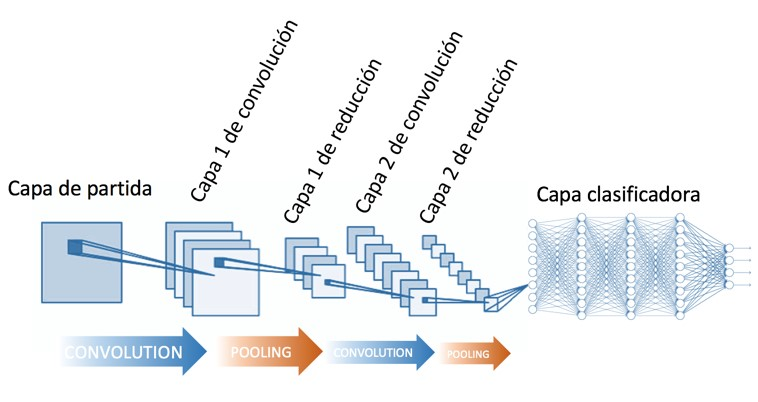
\includegraphics[width=0.50\textwidth]{2/figures/cnn.jpg}
				\caption[Ejemplo de red neuronal convolucional]{Ejemplo de red neuronal convolucional. Fuente: \cite{gl_calvo2017clasifrna}}
				\label{2:fig22}
			\end{center}
		\end{figure}
		
		Hoy en día, las redes neuronales convolucionales tienen múltiples usos desde que la idea fue concebida. Algunos de los problemas en las que pueden ser usados son de clasificación de objetos, recuperación de imágenes, detección y segmentación de objetos, distorsión y filtros de imágenes, por citar los ejemplos más comunes. El modelo de CNN más conocido es “AlexNet” (2012) por ser uno de los pioneros en clasificar imágenes \parencite{tec_li2019cnn}.
		
		Estas redes tienen su origen en el Neocognitron introducido por Fukushima en 1980 como modelo de red neuronal para el mecanismo de reconocimiento de patrón visual sin la enseñanza de un “profesor” (ver Figura \ref{2:fig23}), mismo que en el año 1998 sería mejorado por LeCun, Bottou, Bengio y Haffner al agregar un método de aprendizaje de gradiente aplicado al reconocimiento de documento basado en la propagación hacia atrás (ver Figura \ref{2:fig24}) \parencite{tec_li2019cnn}.
		\begin{figure}[htbp]
			\begin{center}
				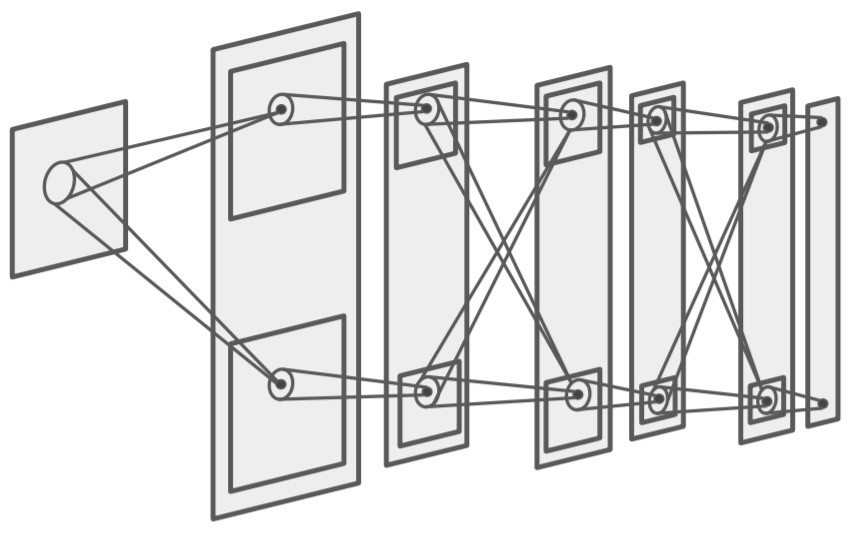
\includegraphics[width=0.6\textwidth]{2/figures/neocognitron.jpg}
				\caption[Modelo Neocognitron de Fukushima (1980)]{Modelo Neocognitron de Fukushima (1980). Fuente: \cite{tec_li2019cnn}}
				\label{2:fig23}
				
				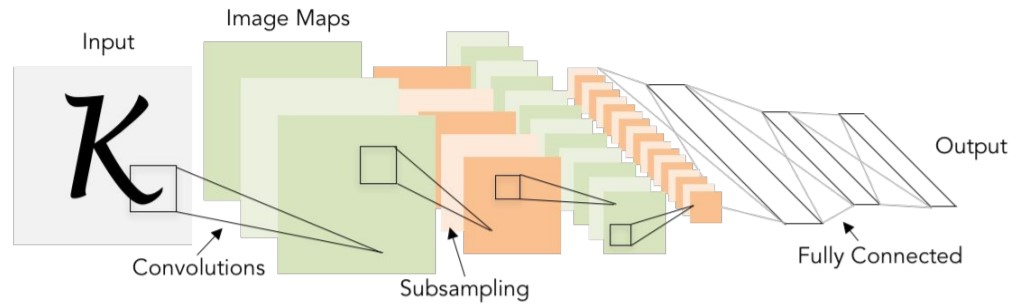
\includegraphics[width=0.8\textwidth]{2/figures/lenet5.jpg}
				\caption[Modelo LeNet-5 de LeCun (1998)]{Modelo LeNet-5 de LeCun (1998). Fuente: \cite{tec_li2019cnn}}
				\label{2:fig24}
			\end{center}
		\end{figure}
		
		Estos modelos se inspiraron en el estudio de la información visual en la corteza donde se ubican hasta 5 áreas. La primera, V1, contiene la información visual donde sus neuronas se ocupan de características visuales de bajo nivel, alimentando así a otras áreas adyacentes. Cada una de ellas se encarga de aspectos más específicos y detallados de la información obtenida. La idea de su implementación es la de solucionar el problema que surgen al escalar imágenes de mucha definición por las redes neuronales ordinarias. Por ello, este tipo de redes trabajan modelando de forma consecutiva piezas pequeñas de información para luego combinarlas en sus capas más profundas \parencite{tec_lopez2016cnnTF}.
		
		Su nombre deriva del concepto convolución. La convolución es un término en las matemáticas usado como operador matemático que convierte dos funciones f y g en una tercera función en donde la primera se superpone a una versión invertida y trasladada de la segunda, así como para denotar la distribución de la función de probabilidad de la suma de dos variables independientes aleatorias. Esta se da por la Ecuación \ref{eq:convolution} \parencite{tec_figueroa_convolucion}:
		\begin{equcaption}[!ht]
			\begin{equation}
			\phantomsection
			(f*g)(t)=\int_0^t f(t-\tau)g(\tau)\mathrm{d}\tau
			\end{equation}
			\caption[Fórmula matemática de la convolución]{Fórmula matemática de la convolución. Fuente: \cite{tec_figueroa_convolucion}}
			\label{eq:convolution}
		\end{equcaption}
		
		Donde el rango puede variar entre un conjunto finito (como en la fórmula desde 0 hasta un valor t) o uno infinito.
		
		La estructura de las Redes Neuronales Convolucionales se constituye en tres tipos de capas \parencite{tec_lopez2016cnnTF}.
		\begin{itemize}
			\item \textbf{Capa convolucional (\textit{Convolutional Layer})}: Es la capa que hace distinta a esta red de otros tipos de redes neuronales artificiales. Se aplica la operación de la convolución, que recibe como entrada (\textit{input} en inglés) a la imagen para luego aplicarle un filtro (\textit{kernel} en inglés), devolviendo un mapa de las características de la imagen original, logrando así reducir el tamaño de los parámetros, como se observa en la Figura \ref{2:fig25}.
			\begin{figure}[h]
				\begin{center}
					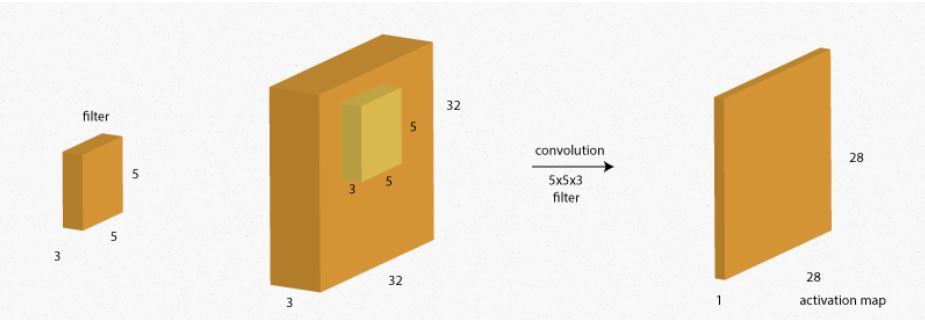
\includegraphics[width=0.8\textwidth]{2/figures/convolucion.jpg}
					\caption[Ejecución de la convolución en una entrada]{Ejecución de la convolución en una entrada. Fuente: \cite{tec_lopez2016cnnTF}}
					\label{2:fig25}
				\end{center}
			\end{figure}
			
			Por ejemplo, en la anterior figura se tiene una imagen de entrada con dimensiones de 32 de alto, 32 de ancho y 3 de profundidad (32x32x3). A ella se le aplica un filtro de dimensiones (5x5x3) que recorrerá toda la imagen para extraer características de cada pixel. Tanto la profundidad de la entrada como del filtro siempre son iguales. El resultado de tomar un producto escalar entre el filtro y un pequeño fragmento de 5x5x3 de la imagen es un número, generando así un mapa de activación de nuevas dimensiones (28x28x1). Por cada n filtros aplicados a la entrada se generan n de estos mapas. Al final, la cantidad de mapas de activación determinará una nueva imagen de n de profundidad, como en la Figura \ref{2:fig26}.
			\begin{figure}[h]
				\begin{center}
					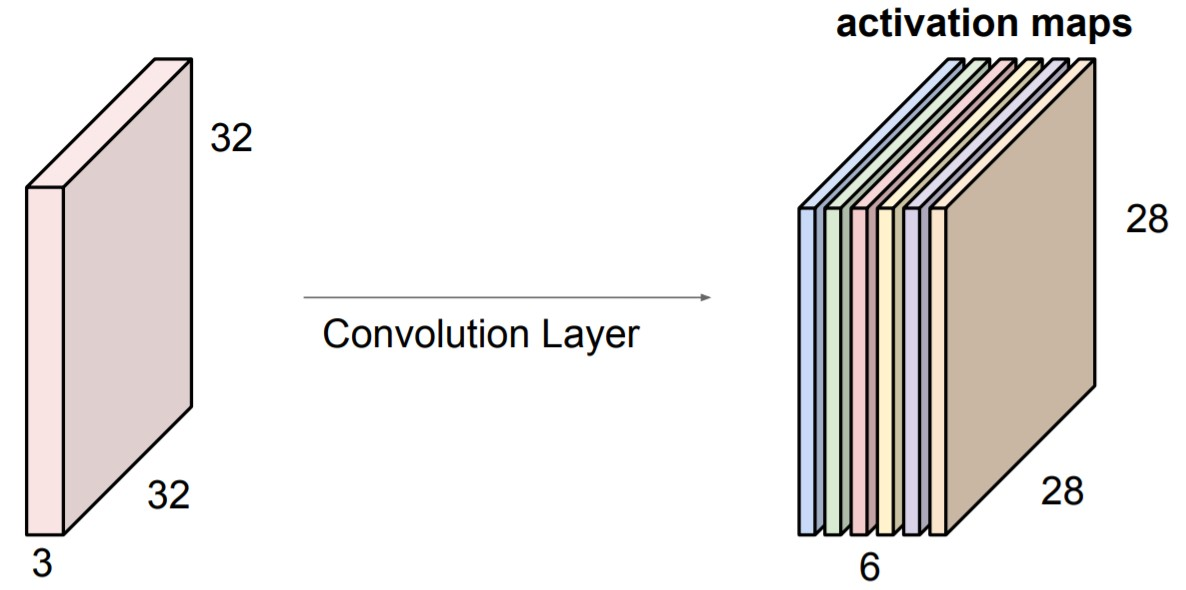
\includegraphics[width=0.7\textwidth]{2/figures/filtros_cnn.jpg}
					\caption[Generación de una nueva imagen a partir de filtros]{Generación de una nueva imagen a partir de filtros. Fuente: \cite{tec_li2019cnn}}
					\label{2:fig26}
				\end{center}
			\end{figure}
			
			Asimismo, cada vez que se aplica una convolución a una imagen, se aplicará una función de activación como en la secuencia de la Figura \ref{2:fig27}.
			\begin{figure}[h]
				\begin{center}
					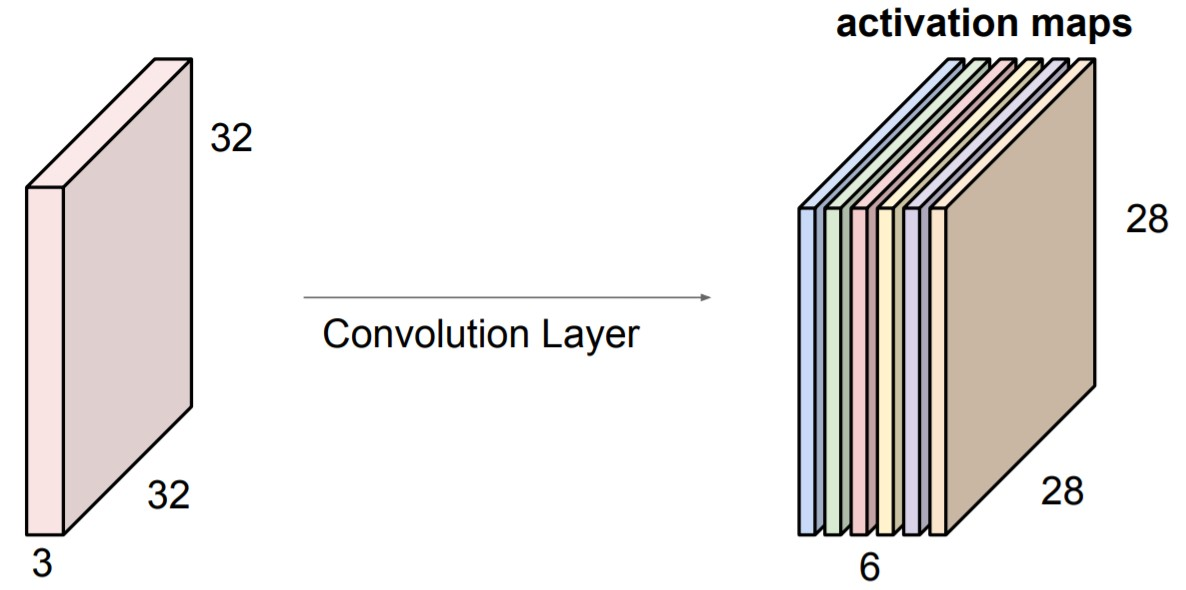
\includegraphics[width=0.60\textwidth]{2/figures/filtros_cnn.jpg}
					\caption[Secuencia de varias capas convolucionales]{Secuencia de varias capas convolucionales. Fuente: \cite{tec_li2019cnn}}
					\label{2:fig27}
				\end{center}
			\end{figure}
			
			A nivel visual, en la Figura \ref{2:fig28} se aprecia un ejemplo de los resultados de aplicar varias convoluciones a una imagen.
			\begin{figure}[h]
				\begin{center}
					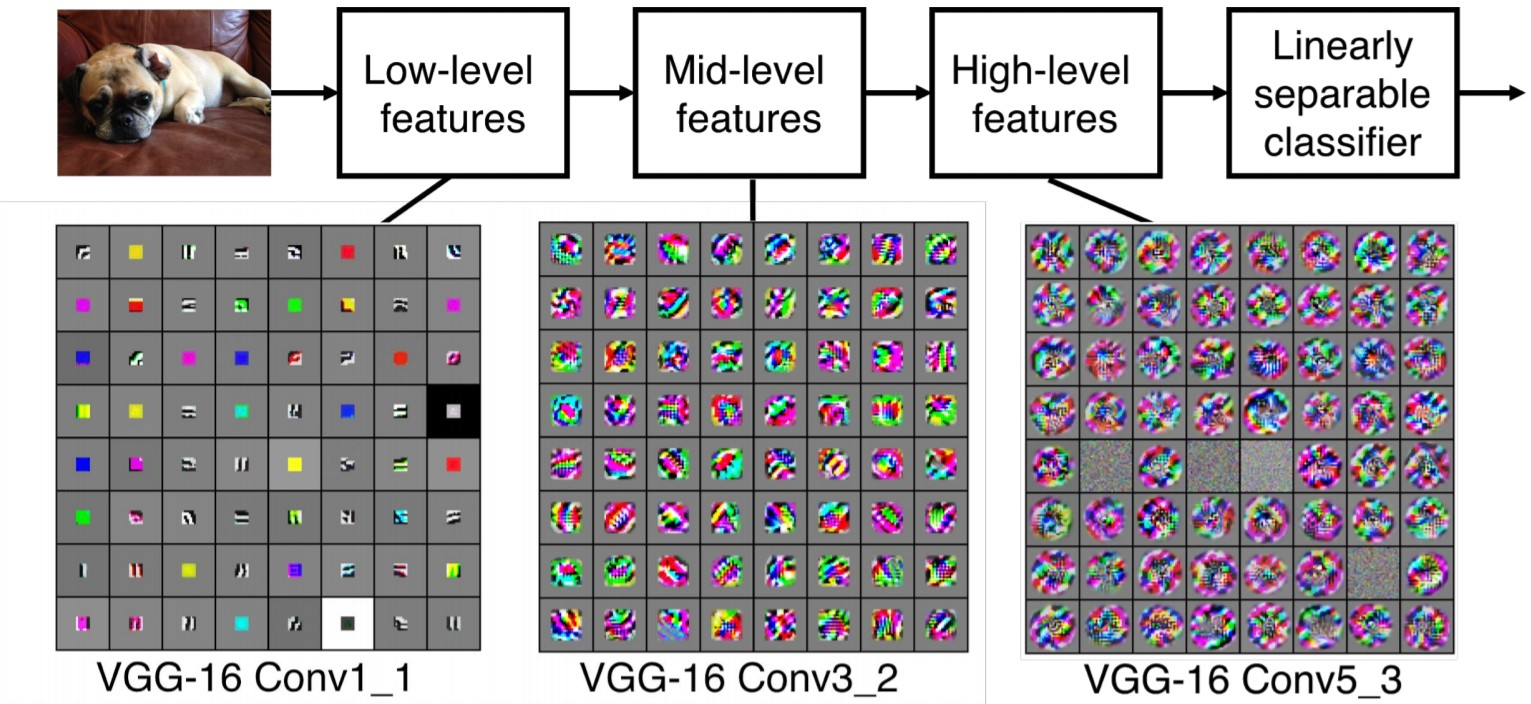
\includegraphics[width=0.70\textwidth]{2/figures/features_cnn.jpg}
					\caption[Extracción de características a partir de convoluciones]{Extracción de características a partir de convoluciones. Fuente: \cite{tec_li2019cnn}}
					\label{2:fig28}
				\end{center}
			\end{figure}
			
			Finalmente, se calcula el volumen de la dimensión de la salida de la Figura \ref{2:fig29} mediante la Ecuación \ref{eq:mapaact}:
			\begin{itemize}
				\item Se tiene una entrada de dimensiones $(h * w * d)$.
				\item Se tiene un filtro de dimensiones $(f_h * f_w * d)$.
			\end{itemize}
			
			\begin{figure}[h]
				\begin{center}
					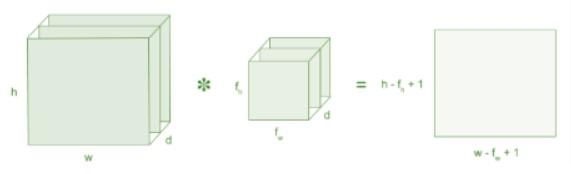
\includegraphics[width=0.75\textwidth]{2/figures/matriz_cnn.jpg}
					\caption[Ejemplo de matriz de imagen de entrada y un filtro]{Ejemplo de matriz de imagen de entrada y un filtro. Fuente: \cite{tec_prabhu2018cnn}}
					\label{2:fig29}
				\end{center}
			\end{figure}
			
			\begin{equcaption}[!ht]
				\begin{equation}
				\phantomsection
				Volumen=(h-f_h+1)*(w-f_w+1)*1
				\end{equation}
				\caption[Cálculo del volumen del mapa de activación]{Cálculo del volumen del mapa de activación. Fuente: \cite{tec_prabhu2018cnn}}
				\label{eq:mapaact}
			\end{equcaption}
			
			\item \textbf{Capa de reducción (\textit{Pooling Layer})}: Esta capa le sucede a la capa convolucional (luego de aplicar la función de activación). Sirve principalmente para reducir las dimensiones espaciales del volumen de la entrada (alto x ancho) para la siguiente capa convolucional. Sin embargo, no afecta la profundidad de la misma. Esta operación que realiza se le conoce también como “reducción de muestreo” debido a que, si bien logra reducir las dimensiones para procesar mejor en la siguiente capa, también conlleva perder información. Por el contrario de lo que se piensa, además de reducir la sobrecarga del cálculo para las siguientes capas, el modelo se beneficia también disminuyendo el sobreajuste.
			
			Para determinar las dimensiones de la nueva imagen generada (siempre que sea cuadrada como en la Figura \ref{2:fig30}) con esta capa, se aplica la Ecuación \ref{eq:outputconv}:
			\begin{figure}[htbp]
				\begin{center}
					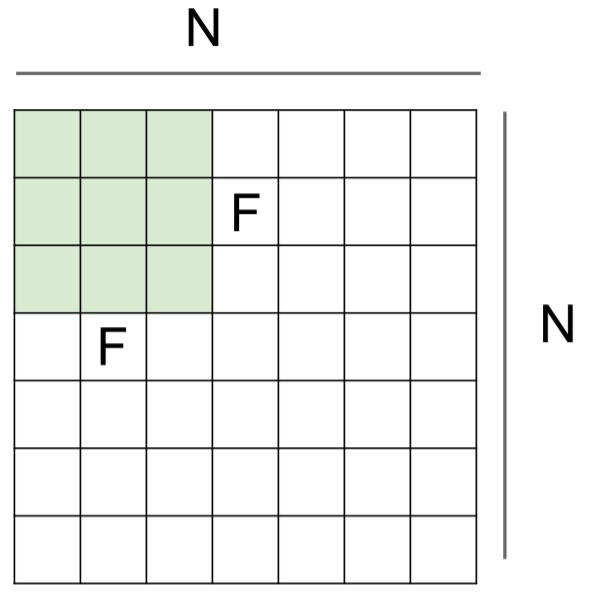
\includegraphics[width=0.3\textwidth]{2/figures/input_filter_cnn.jpg}
					\caption[Dimensiones de una entrada y un filtro]{Dimensiones de una entrada y un filtro. Fuente: \cite{tec_li2019cnn}}
					\label{2:fig30}
				\end{center}
			\end{figure}
		
			\begin{equcaption}[!ht]
				\begin{equation}
				\phantomsection
				Salida=\frac{N-F}{S}+1
				\end{equation}
				\caption[Cálculo del tamaño de la imagen reducida]{Cálculo del tamaño de la imagen reducida. Fuente: \cite{tec_li2019cnn}}
				\label{eq:outputconv}
			\end{equcaption}
		
			Donde:
			\begin{conditions}
				N   &  tamaño del lado de la imagen de entrada \\
				F   &  tamaño del lado del filtro \\   
				S	&  número de desplazamiento de pixeles sobre la matriz de entrada
			\end{conditions}
			
			Por ejemplo, cuando el paso es 1, los filtros se mueven a 1 pixel por vez, cuando el paso es 2, se mueven a 2 píxeles (como en la Figura \ref{2:fig31}) y así sucesivamente \parencite{tec_prabhu2018cnn}.
			\begin{figure}[htbp]
				\begin{center}
					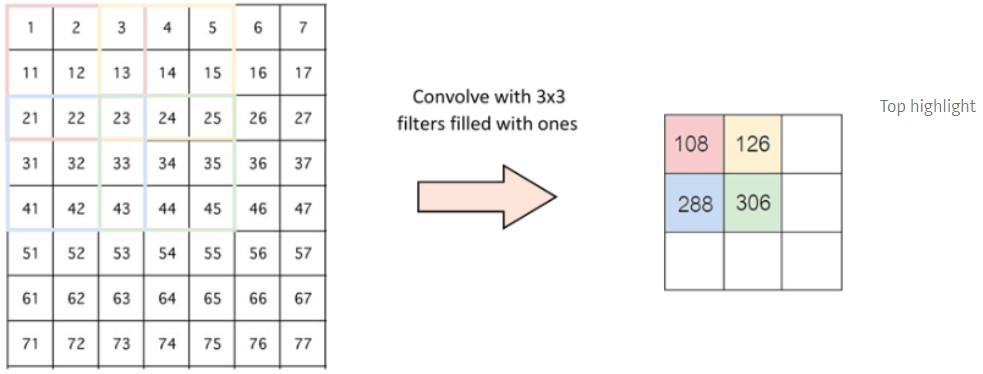
\includegraphics[width=0.60\textwidth]{2/figures/stride_cnn.jpg}
					\caption[Paso de 2 píxeles por parte de un filtro]{Paso de 2 píxeles por parte de un filtro. Fuente: \cite{tec_prabhu2018cnn}}
					\label{2:fig31}
				\end{center}
			\end{figure}
			
			Si, por el contrario, se desea aplicar convolución a una imagen sin afectar sus dimensiones luego de pasar por la capa de reducción, se construye bordes de ceros de n píxeles. A este tamaño de borde se le llama Relleno (\textit{pad} en inglés), por lo que el tamaño de la nueva salida se obtiene mediante la fórmula:
			
			\begin{equcaption}[!ht]
				\begin{equation}
				\phantomsection
				Salida=\frac{N-F+2*Relleno}{S}+1
				\end{equation}
				\caption[Cálculo del tamaño de la imagen reducida con bordes rellenados con ceros]{Cálculo del tamaño de la imagen reducida con bordes rellenados con ceros. Fuente: \cite{tec_li2019cnn}}
				\label{eq:outputconvwithpad}
			\end{equcaption}
			
			Existen diferentes tipos de reducción \parencite{tec_prabhu2018cnn}:
			\begin{itemize}
				\item Max Pooling: Toma el elemento más grande dentro del mapa de características.
				\item Average Pooling: Toma el promedio de los elementos dentro del mapa de características.
				\item Sum Pooling: Toma la suma total de los elementos dentro del mapa de características.
			\end{itemize}
			
			\item \textbf{Capa totalmente conectada (\textit{Fully Connected Layer})}: Al final de las capas de convolución y reducción, se usan redes completamente conectadas a cada pixel considerando que cada uno como una neurona separada al igual que en una red neuronal regular \parencite{tec_lopez2016cnnTF}. En esta capa, se aplana la matriz de todas las características obtenidas anteriormente a un vector y se alinea en una capa completamente conectada a una red neuronal (Figura \ref{2:fig32}).
			\begin{figure}[h]
				\begin{center}
					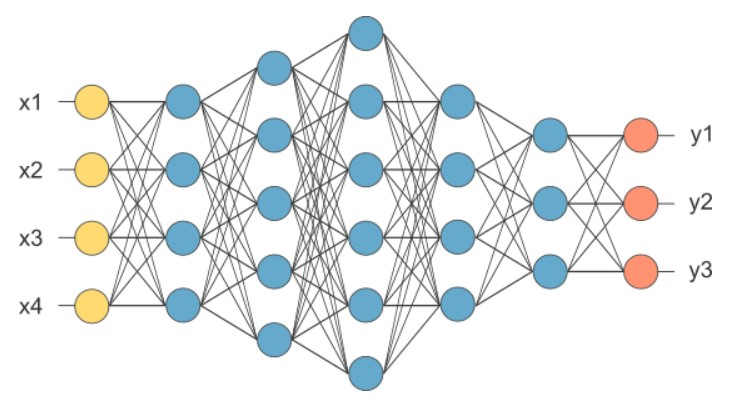
\includegraphics[width=0.60\textwidth]{2/figures/fully_conected_cnn.jpg}
					\caption[Aplanado de matrices luego de agrupar la capa]{Aplanado de matrices luego de agrupar la capa. Fuente: \cite{tec_prabhu2018cnn}}
					\label{2:fig32}
				\end{center}
			\end{figure}
		\end{itemize}
		Para concluir, se muestra a continuación (Figura \ref{2:fig33}) la representación de la arquitectura completa de una Red Neuronal Convolucional resumiendo los conceptos anteriores.
		\begin{figure}[h]
			\begin{center}
				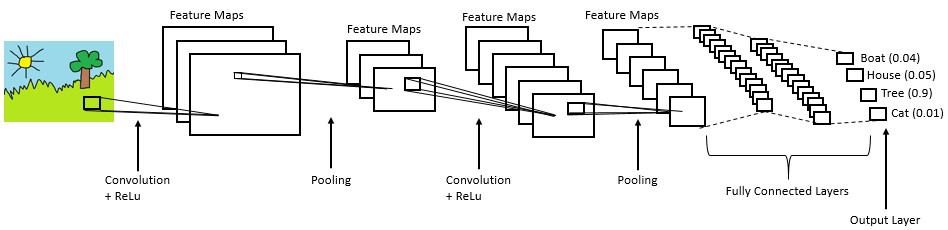
\includegraphics[width=0.8\textwidth]{2/figures/arquitectura_cnn.jpg}
				\caption[Arquitectura completa de una CNN]{Arquitectura completa de una CNN. Fuente: \cite{tec_prabhu2018cnn}}
				\label{2:fig33}
			\end{center}
		\end{figure}
		
		\item \textbf{Redes Neuronales Recurrentes (RNN)}: También conocidas por su nombre en inglés \textit{Recurrent Neural Networks}, se caracterizan por no tener una estructura de capas como se aprecia en la Figura \ref{2:fig34}, sino más bien por permitir conexiones entre sus neuronas de manera arbitraria para crear temporalidad y que toda la red obtenga memoria. Todo esto permite generar una red muy potente para el análisis de secuencias, entre algunos ejemplos se mencionan el análisis de textos, sonidos o video \parencite{gl_calvo2018rnn}.
		\begin{figure}[h]
			\begin{center}
				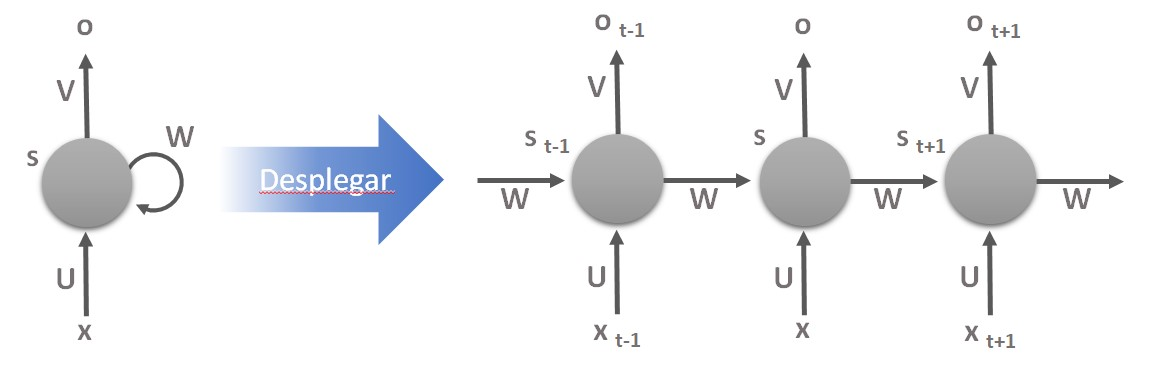
\includegraphics[width=0.8\textwidth]{2/figures/rnn_ejemplo.jpg}
				\caption[Ejemplo de red neuronal recurrente]{Ejemplo de red neuronal recurrente. Fuente: \cite{gl_calvo2018rnn}}
				\label{2:fig34}
			\end{center}
		\end{figure}
	\end{itemize}
	\item \textbf{Máquina de Vectores de Soporte (SVM)}: Es un algoritmo usado para tareas de regresión y clasificación, buscando un hiperplano en un espacio N-dimensional que clasifique claramente los puntos de datos a partir de la distancia máxima entre los puntos de datos de ambas clases. Para ello, maximiza la distancia del margen proporcionando cierto refuerzo para que los puntos de datos futuros puedan clasificarse con más confianza, es decir, que permita distinguir claramente dos clases, como se muestra en la Figura \ref{2:fig35} \parencite{tec_gandhi2018svm}.
	\begin{figure}[h]
		\begin{center}
			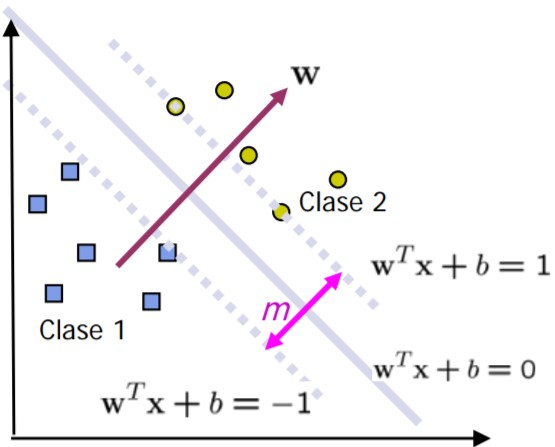
\includegraphics[width=0.45\textwidth]{2/figures/svm_hiperplano.jpg}
			\caption[Hiperplano con dos clases separadas por una distancia m]{Hiperplano con dos clases separadas por una distancia m. Fuente: \cite{tec_betancourt2005svm}}
			\label{2:fig35}
		\end{center}
	\end{figure}
	
	Este algoritmo tiene sus orígenes en la década de los años 60 en Rusia, desarrollados por Vapnik y Chervonenkis. Inicialmente se enfocó en el reconocimiento óptico de caracteres (OCR). Más tarde, los clasificadores de Vectores de Soporte se volvieron competitivos con los mejores sistemas disponibles en ese momento para resolver no solamente el anterior tipo de problema, sino también abarcar tareas de reconocimiento de objetos. En 1998, se publicó el primer manual de estos algoritmos por Burges. Y debido a sus grandes resultados obtenidos en la industria, actualmente se usa con frecuencia en el campo del aprendizaje automático \parencite{tec_smola2004svm}.
	
	Los vectores de soporte hacen referencia a un pequeño subconjunto de las observaciones de entrenamiento que se utilizan como soporte para la ubicación óptima de la superficie de decisión \parencite{gl_mathworks_svm}.
	
	Una Máquina de Vectores de Soporte aprende la superficie decisión de dos clases distintas de los puntos de entrada. Como un clasificador de una sola clase, la descripción dada por los datos de los vectores de soporte es capaz de formar una frontera de decisión alrededor del dominio de los datos de aprendizaje con muy poco o ningún conocimiento de los datos fuera de esta frontera. Los datos son mapeados por medio de un \textit{kernel} Gaussiano u otro tipo de \textit{kernel} a un espacio de características en un espacio dimensional más alto, donde se busca la separación máxima entre clases. Cuando es traída de regreso al espacio de entrada, la función de frontera puede separar los datos en todas las clases distintas, cada una formando un agrupamiento. Esta teoría se basa en la idea de minimización de riesgo estructural (SRM), demostrando en muchas aplicaciones tener mejor desempeño que otros algoritmos de aprendizaje tradicional como las redes neuronales para resolver problemas de clasificación \parencite{tec_betancourt2005svm}.
	
	Cabe mencionar que hay casos en que el conjunto de datos de dos clases puede ser separables no necesariamente de forma lineal. En la Figura \ref{2:fig36} se observan casos linealmente y no linealmente separables, respectivamente.
	\begin{figure}[!ht]
		\centering
		\small
		\begin{subfigure}{.5\textwidth}
			\centering
			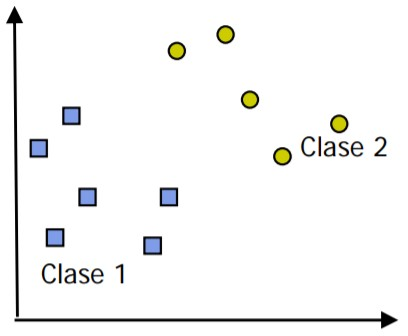
\includegraphics[width=0.6\linewidth]{2/figures/caso1_svm.jpg}
			\caption{Linealmente separable}
		\end{subfigure}%
		\begin{subfigure}{.5\textwidth}
			\centering
			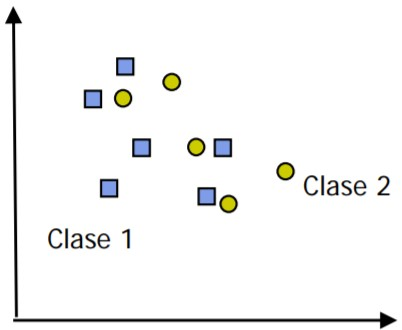
\includegraphics[width=0.6\linewidth]{2/figures/caso2_svm.jpg}
			\caption{No linealmente separable}
		\end{subfigure}
		\caption[Ejemplo de separación de 2 clases]{Ejemplo de separación de 2 clases. Fuente: \cite{tec_betancourt2005svm}}
		\label{2:fig36}
	\end{figure}
	
	
	Lo que se debe hacer para el primer caso es crear el hiperplano a través de una función lineal $w*z+b=0$ y, definido el par $(w,b)$, separar el punto $x_i$ según la Ecuación \ref{eq:hiperplano}:
	
	\begin{equcaption}[!ht]
		\begin{equation}
		\phantomsection
		f(x_i) = sign(w*z+b) =
		\left\{
		\begin{aligned}
		1 \quad y_i=1\\
		-1 \quad y_i=-1
		\end{aligned}
		\right.
		\end{equation}
		\caption[Ecuación del hiperplano para clasificar dos clases]{Ecuación del hiperplano para clasificar dos clases. Fuente: \cite{tec_betancourt2005svm}}
		\label{eq:hiperplano}
	\end{equcaption}
	
	Para el segundo caso, debido a su mayor complejidad, se puede introducir algunas variables no-negativas a la función del hiperplano para hallar su valor óptimo; o también es viable utilizar una función \textit{kernel} que calcule el producto punto de los puntos de entrada en el espacio de características Z, como se aprecia en la Figura \ref{2:fig37}.
	\begin{figure}[h]
		\begin{center}
			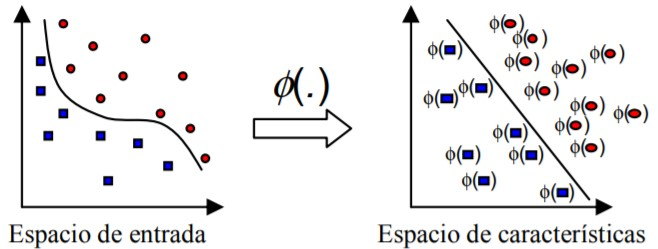
\includegraphics[width=0.7\textwidth]{2/figures/kernel_svm.jpg}
			\caption[Aplicación de un kernel para transformar el espacio de los datos]{Aplicación de un kernel para transformar el espacio de los datos. Fuente: \cite{tec_betancourt2005svm}}
			\label{2:fig37}
		\end{center}
	\end{figure}
	
	\item \textbf{Árboles de Decisión}: Representación visual de decisiones y toma de decisiones utilizada en la minería de datos para derivar una estrategia y alcanzar un objetivo particular. Se dibuja boca abajo con su raíz en la parte superior. Consta de nodos internos, los cuales se subdividen en ramas o bordes y su contenido, las hojas o decisiones \parencite{tec_gupta2017decisiontree}.
	
	Un árbol de decisión toma como entrada un objeto descrito a través de un conjunto de atributos y devuelve una “decisión”. Estos pueden ser discretos o continuos. La salida puede tomar cualquiera de estos dos tipos de valores; en el caso que aprenda una función tomando valores discretos se le denominará clasificación, y en el caso que la función sea continua será llamada regresión. En las clasificaciones booleanas, es decir de dos valores o binaria, clasificará como verdadero (positivo) o falso (negativo). Para alcanzar una decisión, el árbol desarrolla una serie de pruebas a través de sus nodos y las ramas que salen del nodo son etiquetadas con los valores posibles de dicha propiedad. Además, cada nodo hojas del árbol representa el valor que ha de ser devuelto si es alcanzado \parencite{bk_russell2004intart}.
	
	Por ejemplo, representando un ejemplo de este algoritmo, se ilustra en la Figura \ref{2:fig38} para decidir si se debe esperar por una mesa en un restaurante.
	\begin{figure}[h]
		\begin{center}
			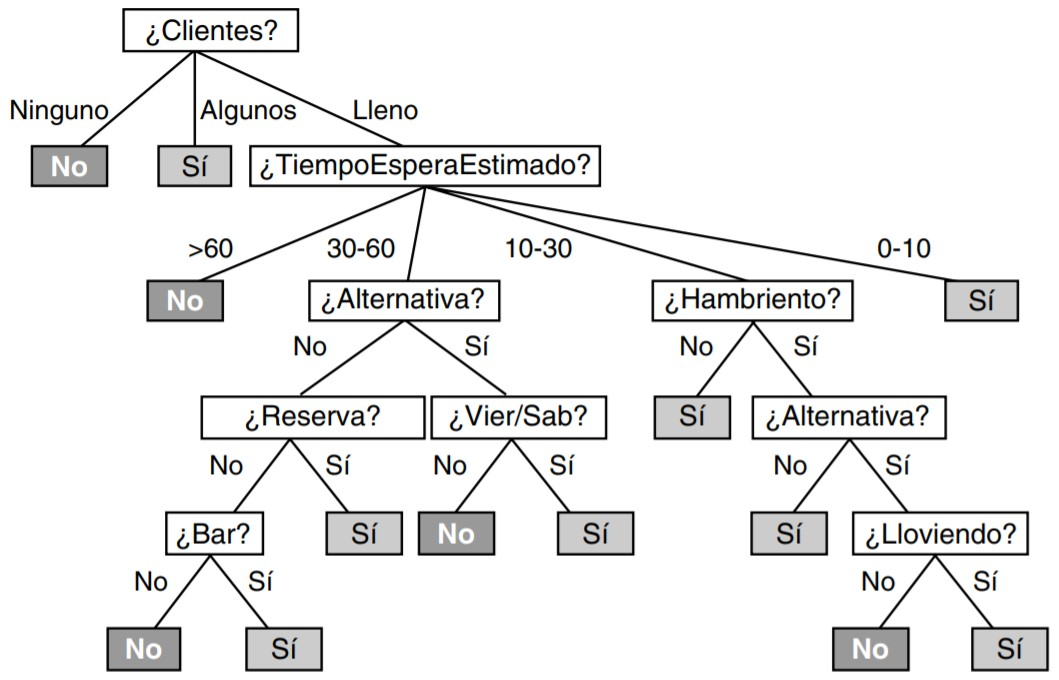
\includegraphics[width=0.8\textwidth]{2/figures/arbol_decision.jpg}
			\caption[Ejemplo del algoritmo de árbol de decisión]{Ejemplo del algoritmo de árbol de decisión. Fuente: \cite{bk_russell2004intart}}
			\label{2:fig38}
		\end{center}
	\end{figure}
\end{itemize}

\clearpage
\subsection{Procesamiento del Lenguaje Natural}
El Procesamiento del Lenguaje Natural (\textit{Natural Language Processing (NLP)} por su nombre en inglés) es un campo interdisciplinario que combina lingüística computacional, ciencias de la computación, ciencia cognitiva e inteligencia artifical. Investiga el uso de las computadoras para entender el lenguaje humano con el fin de realizar tareas útiles, así como lograr una interacción entre ambas partes. Algunas de estas tareas son, por ejemplo, reconocimiento de voz, comprensión del lenguaje hablado, sistemas de diálogo, análisis léxico, análisis de sentimientos, entre otros \parencite{bk_deng2018deeplearningnlp}.

Los autores \citeauthor{bk_deng2018deeplearningnlp} explican en su libro \citetitle{bk_deng2018deeplearningnlp} el desarrollo del estudio de este campo, separando desde una perspectiva histórica en 3 olas: el Racionalismo, el Empiricismo y el Aprendizaje Profundo.

El Racionalismo, nomenclatura establecida entre las décadas de los años 60s y 80s de acuerdo a los argumentos por Noam Chomsky sobre la concepción del lenguaje humano, se basa en el conocimiento de este último fijado por herencia genética y concebido desde el nacimiento. Las primeras apariciones de la aplicación de este enfoque se remontan a la década de los años 50s, donde Alan Turing, en los experimentos que se conocen como "las pruebas de Turing", intentó simular conversaciones de lenguaje natural entre un humano y un computador para generar respuestas similares a la de una persona con el fin de poder evaluar las habilidades que ellas pueden alcanzar. Durante las décadas de los 70s y 80s, los sistemas de entendimiento de lenguaje hablado y sistemas de diálogo se basaron en conjuntos de reglas, desarrollados por la ingeniería de conocimiento experto.

El Empirismo, la segunda ola, se caracterizó por la explotación del cuerpo de texto (\textit{data corpora}) y su uso con Aprendizaje Automático. Esta idea plantea que la mente humana comienza con operaciones de asociación, patrones de reconocimiento y generalización. Algunos ejemplos son el Modelo Ocultro de Markov (HMM) y los modelos de traducción de IBM.

El Aprendizaje Profundo, la tercera y última ola, se basa en el uso de estas técnicas para resolver problemas de Lenguaje Natural que el Aprendizaje Automático no puede lograr para entrenar con grandes cantidades de datos, por ejemplo. Las más comunes son las Redes Neuronales Artificiales, debido a que su configuración permite personalizar la arquitectura basada en múltiples capas e hiperparámetros para soportar el entrenamiento con volúmenes considerables. Sin embargo, pese a sus ventajas, algunas de las limitaciones que presenta son justamente este último detalle para lograr resultados estadísticos impresionantes, mucha capacidad computacional, o habilidades pobres para entender las relaciones de inter-oracional como frases o palabras progresivas dentro de una oración.

Algunas técnicas de Aprendizaje Profundo utilizados actualmente para resolver problemas de NLP comprenden modelos anteriormente mencionados como las Redes Neuronales Convolucionales (CNN) o las Redes Neuronales Recurrentes (RNN). A continuación, se detallarán algunas de las más usadas, así como las principales características y diferencias de ejemplos ya explicados bajo este contexto.

\begin{itemize}
	\item \textbf{Redes Neuronales Convolucionales} (\textit{Convolutional Neural Networks}): Entre las técnicas de minería de datos, se explicaron los conceptos y tipos de Redes Neuronales Artificiales, entre ellas, la actual mencionada. Se comentó que entre sus mayores usos se dan actualmente en el tratamiento de imágenes, problemas de clasificación a partir de estas y visión por computador. El ejemplo más popular fue ImageNet desarrollado por Yann LeCun, informático reconocido por ser el fundador de este tipo de redes, para reconocer objetos dentro de imágenes.
	
	Sin embargo, también son utilizadas para problemas de clasificación de texto. Ronan Collobert y Jason Weston fueron los pioneros de la aplicación de las CNN en tareas de procesamiento de lenguaje natural, modificando y adaptando su arquitectura y parámetros internos \parencite{bk_kamath2019deeplearning_nlp_sr}. En la Figura \ref{2:fig39} se ilustra la arquitectura de una CNN para problemas de NLP.
	\begin{figure}[!ht]
		\begin{center}
			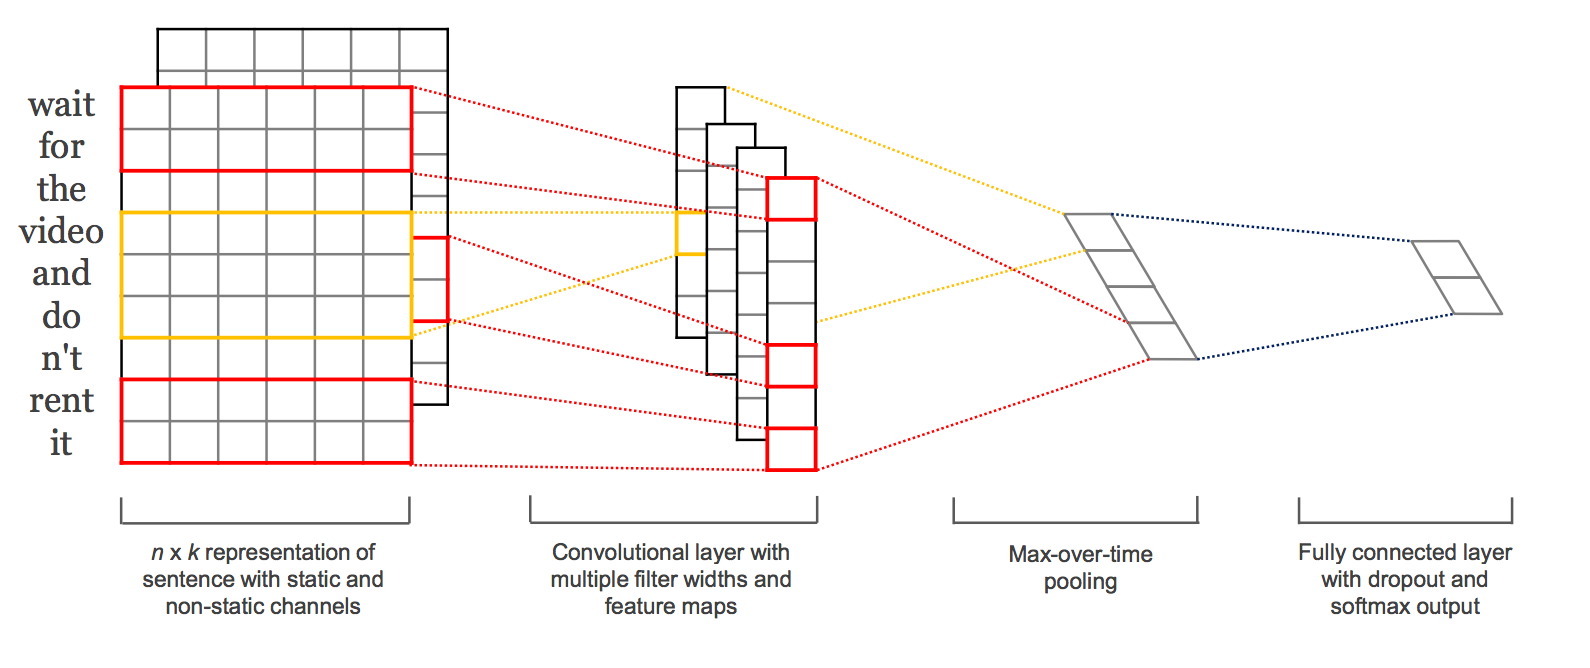
\includegraphics[width=0.8\textwidth]{2/figures/cnn_nlp.png}
			\caption[Arquitectura de modelo CNN con 2 canales para una oración de ejemplo]{Arquitectura de modelo CNN con 2 canales para una oración de ejemplo. Fuente: \cite{tec_kim2014convolutional}}
			\label{2:fig39}
		\end{center}
	\end{figure}
	
	Una de las principales diferencias entre ambos tipos de aplicación es que las convoluciones para imágenes son bidimensionales (2d) debido a que se desplazan a través de matrices de 2 dimensiones (largo y ancho). Mientras que las convoluciones unidimensionales (1d) son muy útiles para series de tiempo y operaciones de NLP por estar conformadas por vectores, aprendiendo así patrones en la dimensión de secuencia \parencite{bk_rao2019nlp_pytorch}. En la Figura \ref{2:fig40} se observa una comparación entre ambos tipos de convolución según el tamaño de dimensión.

	\begin{figure}[!ht]
		\centering
		\small
		\begin{subfigure}{.5\textwidth}
			\centering
			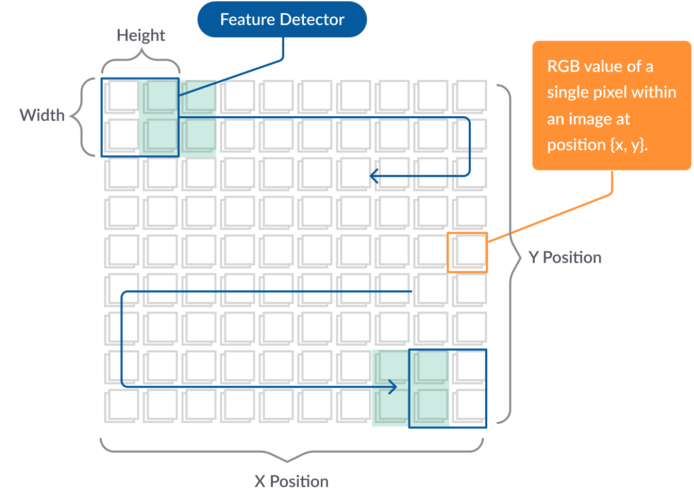
\includegraphics[width=0.85\linewidth]{2/figures/2D-convolutional-example.png}
			\caption{Convolución 2d}
		\end{subfigure}%
		\begin{subfigure}{.5\textwidth}
			\centering
			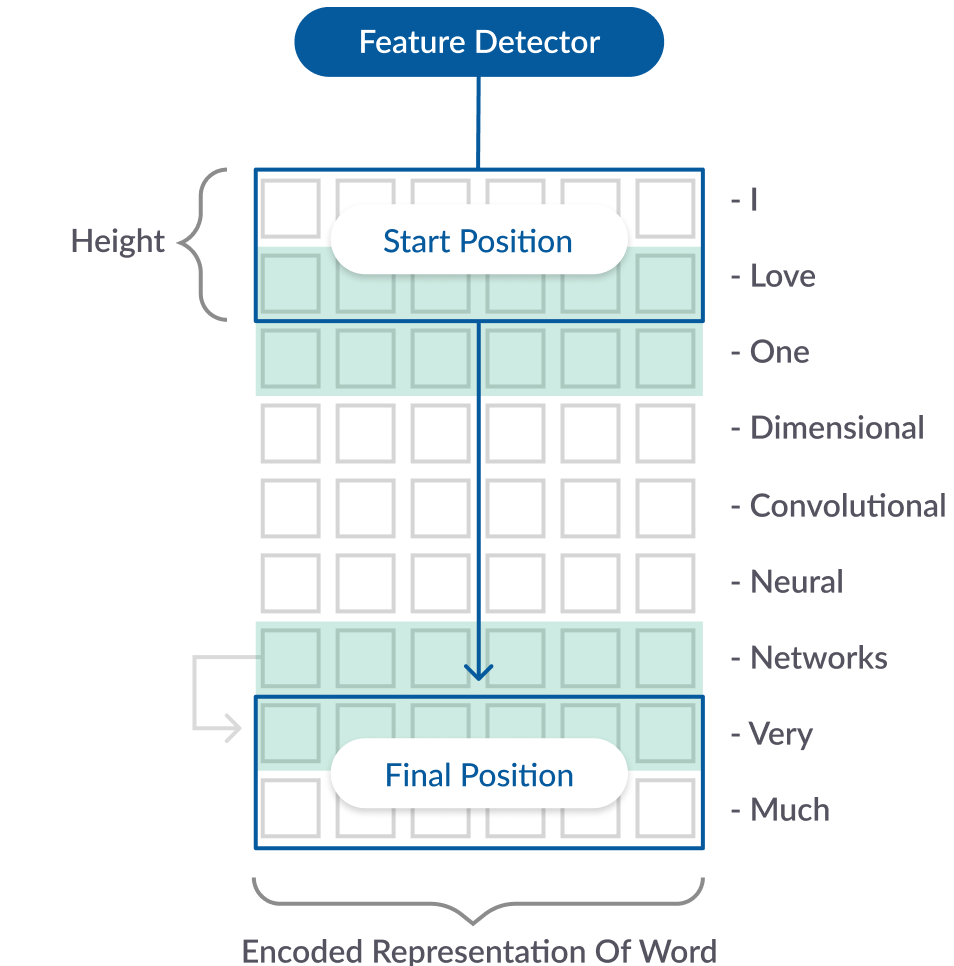
\includegraphics[width=0.70\linewidth]{2/figures/1D-convolutional-example.png}
			\caption{Convolución 1d}
		\end{subfigure}
		\caption[Diferencias entre convoluciones según su dimensión]{Diferencias entre convoluciones según su dimensión. Fuente: \cite{tec_missinglink_conv1d}}
		\label{2:fig40}
	\end{figure}
	
	En la anterior imagen, donde cada palabra codificada se representa por un vector, un kernel de convolución de tamaño de 2 bloques (\textit{kernel\_size}) recorre toda la oración con paso (\textit{stride}) de 1 bloque.
	
	Para problemas de clasificación de texto como los que se considera en esta investigación y en algunos antecedentes con contenido textual, el proceso de la arquitectura CNN de manera general se basa en la Figura \ref{2:fig41}.
	\begin{figure}[!ht]
		\begin{center}
			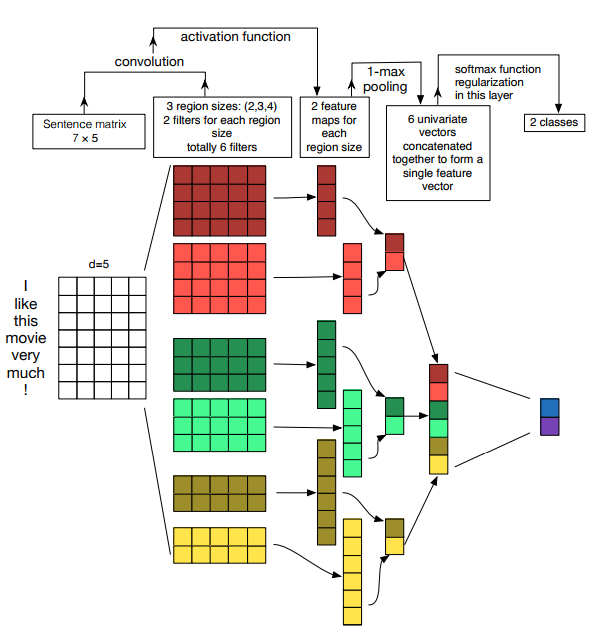
\includegraphics[width=0.40\textwidth]{2/figures/cnn_steps_for_nlp.png}
			\caption[Arquitectura de modelo CNN para clasificación de oraciones]{Arquitectura de modelo CNN para clasificación de oraciones. Fuente: \cite{tec_zhang2017cnn_sentenceclassification}}
			\label{2:fig41}
		\end{center}
	\end{figure}
	
	La idea general es básicamente formar vectores de palabras codificadas para generar una matriz, la cual al ser recorrida por filtros de una dimensión determinada, se obtengan mapas de características para la siguiente entrada. De cada capa resultante, se agruparán (\textit{pooling}) según el criterio del usuario (puede ser valor máximo, mínimo, promedio, etc) para generar nuevos vectores univariantes que serán concatenados y luego el valor final de predicción regularizado entre un rango dependiendo de la función de activación asignada para el problema (\textit{sigmoid} para clasificación de 2 clases o \textit{softmax} a partir de 3 clases). 
	
	\item \textbf{Redes Neuronales Recurrentes} (\textit{Recurrent Neural Networks}): Este tipo de redes también fue comentada brevemente en los tipos de redes neuronales más conocidas. Las RNN son muy usadas incluso también en series de tiempo, ya que los datos para estas casuísticas son secuencias, es decir, una colección ordenada de elementos. Para el caso del lenguaje humano, en donde el habla es un conjunto de secuencia de palabras llamadas fonemas, se busca predecir la siguiente palabra en una oración dada a partir de un elemento dependiente, en este caso, las palabras previas \parencite{bk_rao2019nlp_pytorch}. Como ejemplos de estos casos de uso más comunes se mencionan a los motores de búsqueda en navegadores o sitios web, traductores, entre otros.
	
	Según \cite{bk_brownlee2017deeplearning_nlp}, las RNN generalmente más usadas son los siguientes 3 tipos:
	\begin{itemize}
		\item \textbf{RNN Simple} (\textit{Elman Network} o S-RNN): Son el tipo de redes neuronales recurrentes más básicas, propuesto por Jeffrey L. Elman en 1990, cuya arquitectura se caracteriza por la secuencia de elementos, como en la Figura \ref{2:fig35}.
		Las S-RNN proporcionan resultados sólidos para el etiquetado de secuencias, así como para el modelado del lenguaje.
		
		La ecuación para representar un estado determinado en una RNN toma la siguiente forma:
		
		\begin{equcaption}[!ht]
			\begin{equation}	
			\phantomsection
			s_i = R_{SRNN}(x_i, s_{i-1}) = g([s_{i-1};x_i]W+b)
			\end{equation}
			\caption[Fórmula para determinar un estado en una S-RNN]{Fórmula para determinar un estado en una S-RNN. Fuente: \cite{bk_brownlee2017deeplearning_nlp}}
			\label{eq:srnn}
		\end{equcaption}
		
		Donde se observa que un estado depende de la información del estado previo.
		
		\item \textbf{Memoria Larga a Corto Plazo} (\textit{Long-Short Term Memory} o LSTM): Este modelo fue desarrollado para encargarse del problema de los gradientes que desaparecen de la RNN Simple, que limitaba más adelante el entrenamiento de las RNN profundas.
		
		Según el mismo autor, este problema surge debido a que los gradientes incluyen la multiplicación repetida de la matriz W (de la Ecuación \ref{eq:srnn}), haciendo que los valores desaparezcan.
		
		Esta arquitectura divide el vector de un estado observado $s_i$ en dos mitades, donde una es tratada como “celdas de memoria” y la otra es la memoria de trabajo. Las del primer grupo tienen como función preservar la memoria, así como también los gradientes de error, a lo largo del tiempo. Son controladas mediante componentes de puerta diferenciables, que son funciones matemáticas suaves simuladoras puertas lógicas. En cada estado de entrada, se utiliza una puerta para decidir qué cantidad de la nueva entrada se debe escribir en la memoria.
		
		La arquitectura LSTM es actualmente la más exitosa dentro de las RNN. Un ejemplo de su representación puede ilustrarse en la Figura \ref{2:fig42}.
		
		\begin{figure}[!ht]
			\begin{center}
				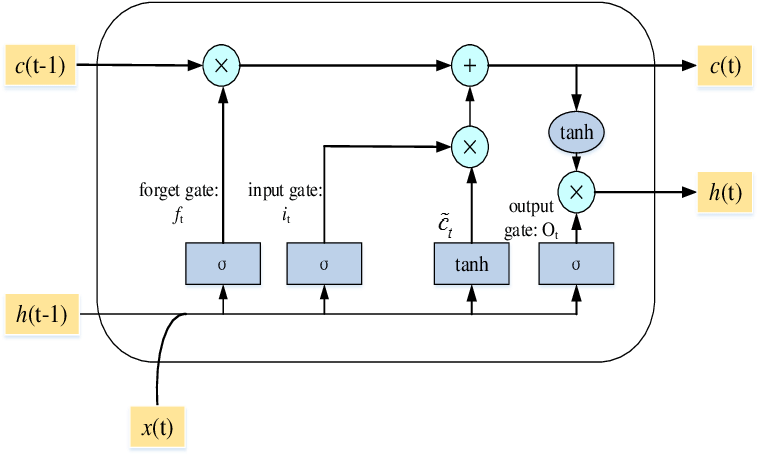
\includegraphics[width=0.6\textwidth]{2/figures/lstm.png}
				\caption[Arquitectura de una LSTM]{Arquitectura de una LSTM. Fuente: \cite{tec_yuan2019lstm}}
				\label{2:fig42}
			\end{center}
		\end{figure}
	
		En donde $x$ son las entradas, $c_{t-1}$ y $c_{t}$ los estados de la celda, y $h_{t-1}$ y $h_{t}$  las salidas.
		
		Una variante muy útil de las RNN son las RNN Bidireccionales (\textit{Bidirectional RNN} o \textit{BiRNN}). Mientras una red neuronal recurrente toma una palabra del pasado para predecir el siguiente, las bidireccionales permiten mirar arbitrariamente lejos tanto al pasado como al futuro dentro de una secuencia \parencite{bk_goldberg2017nn_nlp}.
		La ventaja que se logra a partir de estas características es que, por ejemplo, el modelo puede identificar y discernir mejor en la predicción de la siguiente palabra en el caso de existir 2 o más secuencias idénticas (problema de reconocimiento de entidades nombradas) al lograr conocer más información.
		
		\citeauthor{tec_ng2018bidirectionalRNN}, fundador de Coursera, DeepLearning.AI, Landing AI y Google Brain, explica lo anterior con el siguiente ejemplo como parte del curso Redes Neuronales Recurrentes \parencite{tec_ng2018bidirectionalRNN}:
		
		Sean las oraciones \textit{He said, “Teddy bears are on sale!”} y \textit{He said, “Teddy Roosevel was a great President!”}, se desea saber si \textit{Teddy} es parte del nombre de una persona. El problema es que se cuenta con 2 oraciones cuya secuencia inicial de 3 palabras resultan ser las mismas, pero con distinto panorama posterior a estas. Por ello, la red es duplicada pero con orden de secuencia invertida y colocada en paralelo con la original para que cada una de las nuevas capas conecten sus salidas con las pre-existentes y originen una nueva predicción que toma información previa y posterior.
		
		Bajo la misma premisa, pero con la oración de ejemplo \textit{The brown fox jumped over the dog}, se representa la arquitectura de una BiRNN en la Figura \ref{2:fig43}.
		
		\begin{figure}[!ht]
			\begin{center}
				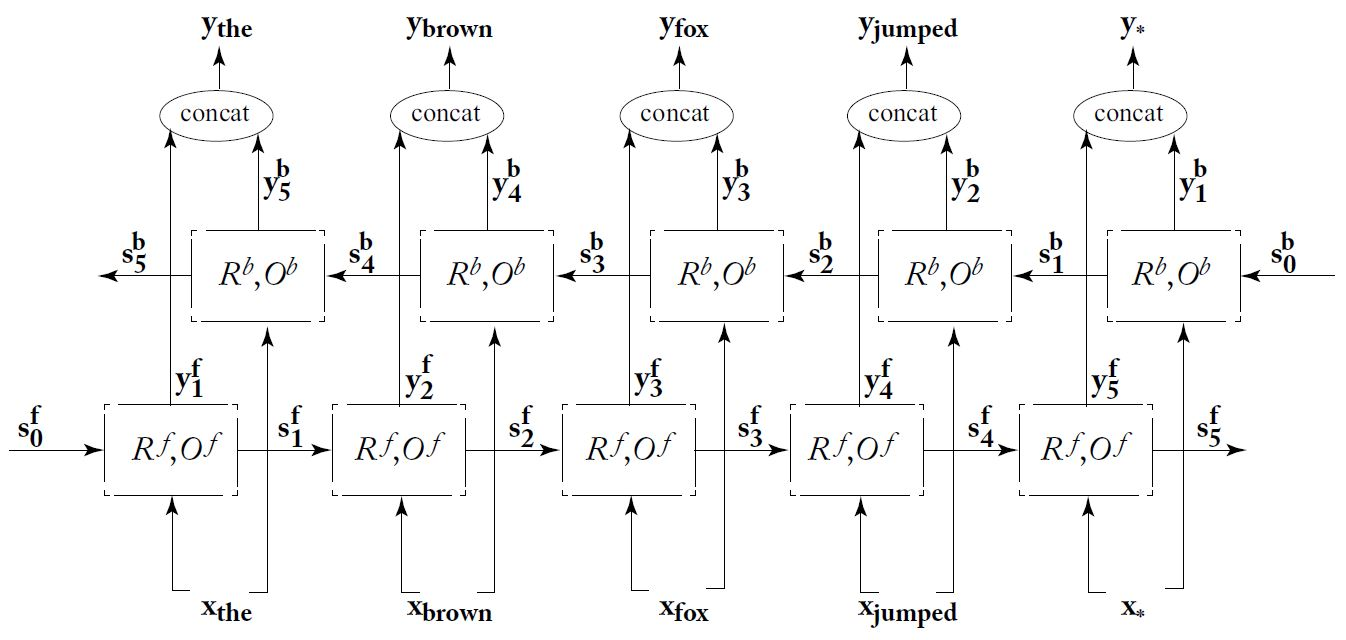
\includegraphics[width=0.8\textwidth]{2/figures/birnn_architecture.jpg}
				\caption[Representación de arquitectura BiRNN de la palabra \textit{jumped} en la oración]{Representación de arquitectura BiRNN de la palabra \textit{jumped} en la oración. Fuente: \cite{bk_goldberg2017nn_nlp}}
				\label{2:fig43}
			\end{center}
		\end{figure}
		
		Como parte de las BiRNN, se encuentra la LSTM Bidireccional (\textit{Bidirectional LSTM} o \textit{BiLSTM}), mejora de la LSTM, que sobresale particularmente en la representación de palabras en la secuencia junto con sus contextos, capturando la palabra y las incontables posibilidades existentes a su alrededor \parencite{bk_deng2018deeplearningnlp}.
		
		\item \textbf{Unidad Recurrente Cerrada} (\textit{Gated Recurrent Unit} o GRU): Este modelo se desarrolló con la intención de simplificar la LSTM debido a su complejidad. Al igual que esta, consiste en un mecanismo de puertas pero en menor cantidad y sin un componente de memoria separada (ver Figura \ref{2:fig44}). La red GRU muestra ser efectiva en modelamiento de lenguaje y máquina traductora \parencite{bk_goldberg2017nn_nlp}.
		
		\begin{figure}[!ht]
			\begin{center}
				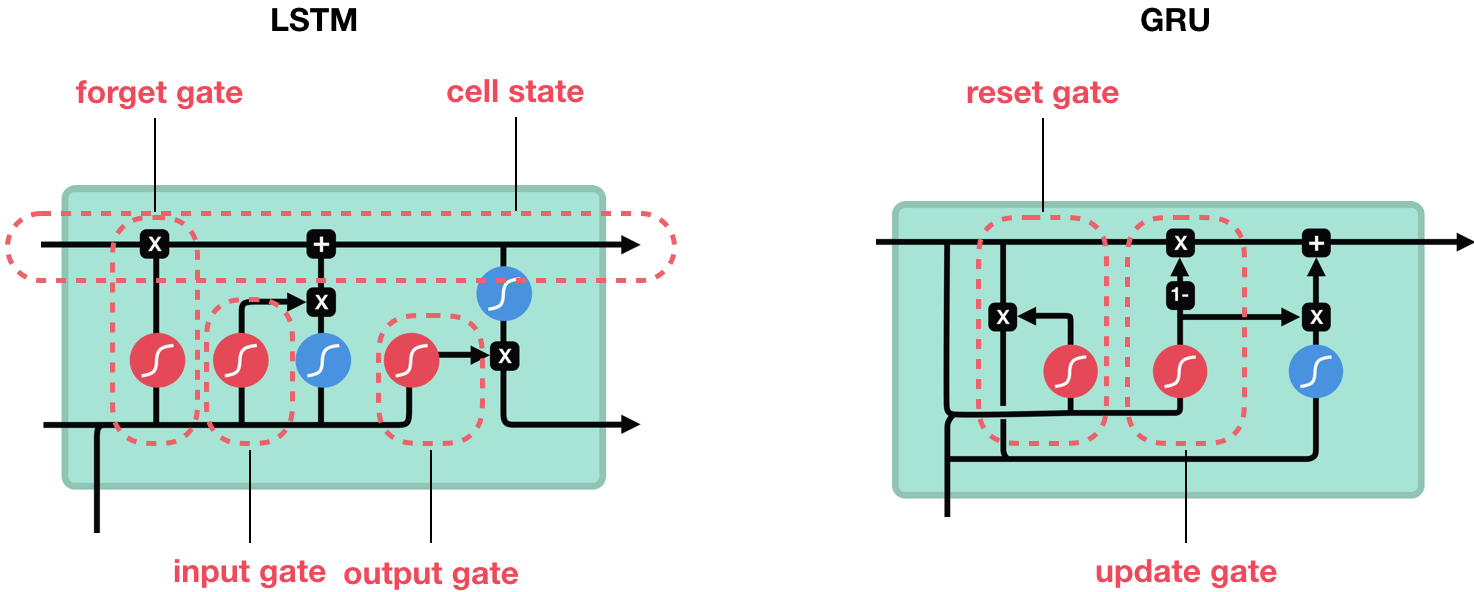
\includegraphics[width=0.8\textwidth]{2/figures/lstm_vs_gru.png}
				\caption[Comparación entre arquitecturas LSTM y GRU]{Comparación entre arquitecturas LSTM y GRU. Fuente: \cite{tec_phi2018gru}}
				\label{2:fig44}
			\end{center}
		\end{figure}
		
		Sin embargo, al compararse los resultados entre estos 3 tipos de modelos, por lo general el mejor desempeño tiene la LSTM \parencite{bk_brownlee2017deeplearning_nlp}.
	\end{itemize}
	
	\item \textbf{Modelo Secuencia a Secuencia} (\textit{Sequence-to-Sequence Model} o \textit{Seq2seq Model}): También conocida como \textit{Encoder-Decoder} (Codificador-Decodificador por su traducción al español), es un tipo de generador de lenguaje natural (\textit{Natural Language Generation} o NLG) usado comúnmente para traducción (por ejemplo, Google Traductor). Se basa en 2 capas LSTM, en donde la primera es usada para codificar la oración de entrada en un “vector de pensamiento”, y la otra para decodificar en una respuesta (ver Figura \ref{2:fig45}) \parencite{bk_deng2018deeplearningnlp}.
	
	\begin{figure}[!ht]
		\begin{center}
			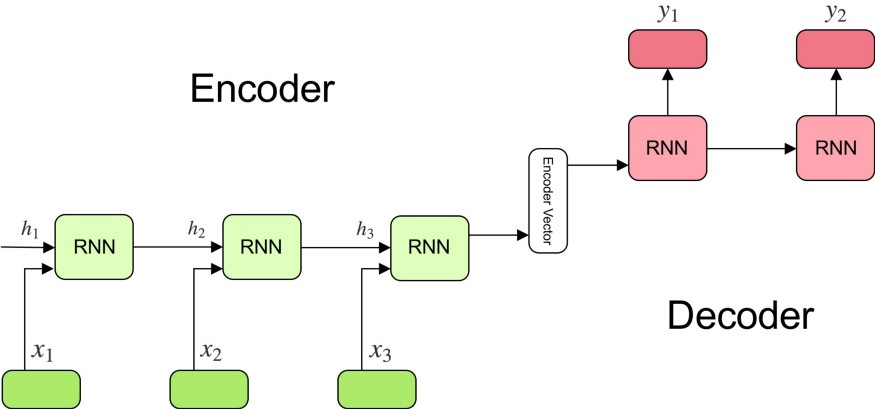
\includegraphics[width=0.7\textwidth]{2/figures/encoder-decoder.jpeg}
			\caption[Arquitectura de un modelo Seq2seq]{Arquitectura de un modelo Seq2seq. Fuente: \cite{tec_kostadinov2019seq2seq}}
			\label{2:fig45}
		\end{center}
	\end{figure}
	
	\item \textbf{Aprendizaje Profundo Multimodal y Multitarea} (\textit{Multimodal and Multitask Deep Learning}): Son un tipo de aprendizaje basado en la explotación de representaciones latentes en las redes neuronales profundas agrupando distintas modalidades (por ejemplo, audio, imágenes, texto, videos, etc) o múltiples tareas (predicción, clasificación, series de tiempo, entre otros) como en la Figura \ref{2:fig46} \parencite{bk_deng2018deeplearningnlp}
	
	\begin{figure}[!ht]
		\begin{center}
			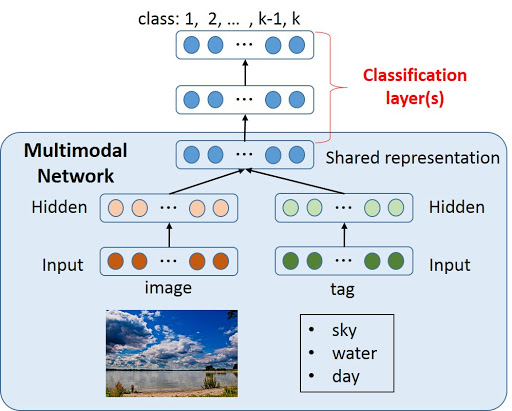
\includegraphics[width=0.50\textwidth]{2/figures/multimodal_network.jpg}
			\caption[Arquitectura de un modelo multimodal de imágenes y texto]{Arquitectura de un modelo multimodal de imágenes y texto. Fuente: \cite{tec_nishida2015multimodal}}
			\label{2:fig46}
		\end{center}
	\end{figure}
	
\end{itemize}

El contenido textual que se usa en los modelos anteriores debe ser pre-procesada previamente. El texto en sí no puede ser incluido tal cual en los modelos de Aprendizaje Automático o Aprendizaje Profundo sin antes ser limpiado \parencite{bk_brownlee2017deeplearning_nlp}. Python ofrece una librería para trabajar y modelar texto llamada Natural Language Toolkit o NLTK. Algunas de las funciones disponibles se encuentran separación de texto en oraciones, separación en palabras o tokenización, eliminación de signos de puntuación, eliminación de palabras de parada (\textit{stop words}), reducción de palabras hacia su forma raíz (\textit{stemming}), retorno de palabras hacia su base o forma diccionario (\textit{lemmatization}).

Suprimir contenido como signos de puntuación, caracteres especiales, palabras de parada, enlaces web, entre otros, ayuda a reducir la cantidad de vectores innecesarios para las representaciones de palabras que se utilizan en la fase de entrenamiento. Para ello, la secuencia de entrada debe dividirse en \textit{tokens}, que pueden ser una palabra, oración, párrafo.

NLTK ofrece más de una alternativa para la tokenización, como por ejemplo, \textit{WhitespaceTokenizer} (elimina espacios en blanco para separar palabras y signos de puntuación en una oración, estos últimos no son independientes), \textit{TreebankWordTokenizer} (separa palabras y signos de puntuación en una oración de manera independiente) y \textit{WordPunctTokenizer} (funciona igual que TreebankWordTokenizer pero no distingue contracciones en idiomas como el inglés). La elección de alguna de estas depende del objetivo que busque el usuario. Asimismo, la reducción de palabras hacia su raíz (llamada \textit{stem}) permite suprimir los prefijos o sufijos agregados a una palabra. Sin embargo, presenta problemas en formas irregulares, generando “No palabras”. El retorno de palabras hacia su forma base (llamada \textit{lemma}), por su lado, convertir palabras conjugadas en distintas variantes de tiempo. Aún así, no todas las formas pueden ser reducidas. La finalidad de estos 2 últimos es reducir una palabra a su forma más primitiva (expresiones regulares) para generar un diccionario homogéneo \parencite{tec_zimovnov2018text_preprocessing}.

Luego de la limpieza de texto, el nuevo conjunto de datos debe representarse como vectores. Dentro de las modalidades más usadas para representación de palabras se encuentran:
\begin{itemize}
	\item \textbf{Incrustación de palabra} (\textit{Word Embedding}): Es una representación aprendida para texto en donde las palabras con el mismo significado tienen una similar representación. La principal ventaja que presenta es la baja dimensionalidad de vectores a nivel computacional, ya que una palabra individual se representa como vectores de valor real en un espacio vectorial predefinido, a diferencia de otros métodos de muy alta dimensionalidad como la codificación en caliente (\textit{one hot encoding}) o la bolsa de palabras (\textit{bag-of-words}), en donde distintas palabras presentan diferentes representaciones \parencite{bk_brownlee2017deeplearning_nlp}.
	
	Algunos de los algoritmos destacados de este grupo son:
	\begin{itemize}
		\item \textbf{Capa de incrustación} (\textit{Embedding Layer}): Consiste en una incrustación de palabras que aprende con un modelo de red neuronal. En esta capa, se especifica el tamaño del espacio vectorial (dimensiones), donde los vectores inicializan con pequeños valores aleatorios. La capa se utiliza en el extremo frontal de la red, es decir, luego de la capa de entrada, y es ajustada de forma supervisada mediante el algoritmo de propagación hacia atrás. Puede recibir palabras codificadas, en donde cada una se representa por un código, o codificación en caliente, la cual presenta mayor dimensión. Si se utiliza un Perceptrón Multicapa (MLP), los vectores de palabras son concatenados antes de entrar al modelo. En el caso se use una RNN, cada palabra será tomada como una entrada en una secuencia \parencite{bk_brownlee2017deeplearning_nlp}. Como se observa en la Figura \ref{2:fig47}, la capa de incrustación toma como entrada a la matriz de incrustación y la transforma en un vector tridimensional de \textit{n} registros.
		
		\begin{figure}[!ht]
			\begin{center}
				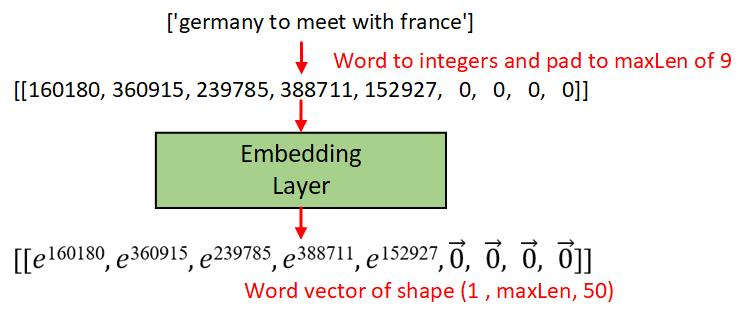
\includegraphics[width=0.50\textwidth]{2/figures/embedding_layer.jpg}
				\caption[Ejemplo de funcionamiento de una capa de incrustación]{Ejemplo de funcionamiento de una capa de incrustación. Fuente: \cite{tec_chengwei2018embedding}}
				\label{2:fig47}
			\end{center}
		\end{figure}
		
		\item \textbf{Palabra a vector} (\textit{Word2Vec}): Se trata de un método estadístico, desarrollado en el 2013 por Tomas Mikolov, cuya finalidad es de aprender eficientemente una incrustación de palabras independientes de un corpus de texto, incluso si este y sus dimensiones son más grandes. En este trabajo se involucró el análisis de los vectores aprendidos y la exploración de la matemática vectorial para representar palabras. Para entender estos conceptos, se ilustra bajo el ejemplo de la analogía “\textit{Rey es a Reina como hombre es a mujer}”, en donde se evidencia la relación sintáctica y semántica capturada por su proximidad vectorial \parencite{bk_brownlee2017deeplearning_nlp}. La Figura \ref{2:fig48} grafica las palabras relacionadas en un espacio vectorial gracias al algoritmo.
		
		\begin{figure}[!ht]
			\begin{center}
				\includegraphics[width=0.60\textwidth]{2/figures/word2vec.png}
				\caption[Incrustaciones de palabras por Word2Vec]{Incrustaciones de palabras por Word2Vec. Fuente: \cite{tec_bujokas2020word2vec}}
				\label{2:fig48}
			\end{center}
		\end{figure}
		
		\item \textbf{Vectores globales para representación de palabra} (\textit{GloVe}): Es un algoritmo de aprendizaje no supervisado para obtener representaciones vectoriales de palabras. Es una extensión del método Word2Vec, desarrollado en 2014 por Jeffrey Pennington como proyecto de código abierto en la Universidad Stanford. Las representaciones de palabras del modelo de espacio vectorial clásico se desarrollaron utilizando técnicas de factorización matricial como el Análisis semántico latente (LSA), con el cual combina sus características de aprendizaje adoptadas de Word2Vec, logrando un modelo de aprendizaje con mejor performance para incrustación de palabras \parencite{gl_pennington2014glove}. GloVe dispone en su web distintos vectores de palabras pre-entrenados, entre ellas, un vocabulario de más de 400 mil palabras, hasta 4 opciones de matrices con distintas dimensiones, y 6 billones de tokens extraídos de Wikipedia (2014) y Gigaword (5ta edición) de la Universidad de Pensilvania, así como datas públicas extraídas de mayor tamaño. La Figura \ref{2:fig49} ilustra ejemplos de palabras  relacionadas en un espacio vectorial gracias al algoritmo. La relación semántica (palabras clasificadas en un mismo grupo) entre ellas se aprecia por la cercanía en su el eje Y. Mientras que aquellos señalados con líneas horizontales en su eje X se encuentran asociadas por analogías, como por ejemplo, género, geolocalización, compañía, grados del adjetivo, entre otros.
		
		\begin{figure}[!ht]
			\centering
			\small
			\begin{subfigure}{.55\textwidth}
				\centering
				\includegraphics[width=0.70\linewidth]{2/figures/glove_man-woman.jpg}
				\caption{hombre - mujer}
			\end{subfigure}%
			\begin{subfigure}{.55\textwidth}
				\centering
				\includegraphics[width=0.70\linewidth]{2/figures/glove_company-ceo.jpg}
				\caption{compañía - CEO}
			\end{subfigure}
			\begin{subfigure}{.55\textwidth}
				\centering
				\includegraphics[width=0.70\linewidth]{2/figures/glove_comparative-superlative.jpg}
				\caption{comparativo - superlativo}
			\end{subfigure}%
			\begin{subfigure}{.55\textwidth}
				\centering
				\includegraphics[width=0.70\linewidth]{2/figures/glove_city-zipcode.jpg}
				\caption{ciudad - código postal}
			\end{subfigure}
			\caption[Incrustaciones de palabras por GloVe]{Incrustaciones de palabras por GloVe. Fuente: \cite{tec_pennington2014glove}}
			\label{2:fig49}
		\end{figure}
		
	\end{itemize}

	\item \textbf{Bolsa de palabras} (\textit{Bag-of-Words} o \textit{BoW}): Consiste en una forma de extraer características de textos implicando un vocabulario de palabras conocidas y una métrica de presencia de éstas. Se le denomina Bolsa de palabras ya que no considera el orden o la estructura de las palabras dentro del documento, sólo se enfoca en conocer su presencia. El algoritmo relaciona la similitud entre documentos si tienen contenido similar \parencite{bk_brownlee2017deeplearning_nlp}. Por ejemplo, en la Figura \ref{2:fig50} el algoritmo cuantifica la frecuencia cada palabra individual dentro de un documento sin importar su orden. De esta manera, los relaciona a partir de su recurrencia en todos ellos
	
	\begin{figure}[!ht]
		\begin{center}
			\includegraphics[width=0.70\textwidth]{2/figures/bow_example.png}
			\caption[Ejemplo de funcionamiento de bolsa de palabras]{Ejemplo de funcionamiento de bolsa de palabras. Fuente: \cite{tec_zhou2019bow}}
			\label{2:fig50}
		\end{center}
	\end{figure}
	
	\item \textbf{Frecuencia del término - Frecuencia inversa del documento} (\textit{Term Frequency - Inverse Document Frequency} o \textit{TF-IDF}): Es un algoritmo que también contabiliza palabras pero que resaltan aquellas más significativas para calcular sus pesos correspondientes. Se compone por la frecuencia del término, que representa la frecuencia con la que una palabra determinada aparece en un documento, y la frecuencia inversa del documento, el cual reduce la escala de palabras que aparecen mucho en los documentos \parencite{bk_brownlee2017deeplearning_nlp}. Su peso se calcula bajo la siguiente fórmula:
	
	\begin{equcaption}[!ht]
		\begin{equation}
		\phantomsection
		TF-IDF_{(n,d)}=TF_{(n,d)}*IDF_{(n)}
		\end{equation}
		\caption[Fórmula de TF-IDF]{Fórmula de TF-IDF. Fuente: \cite{tec_hamdaoui2019tfidf}}
		\label{eq:tfidf}
	\end{equcaption}
	
	Donde:
	\begin{conditions}
		TF_{(n,d)}	&	número de veces que el término \textit{t} aparece en un documento \textit{d} \\
		IDF_{(n)}	&	$\log{\frac{1+n}{1+df_{(d,n)}}+1}$	\\
		n			&	número de documentos	\\
		df_{(d,n)}	&	frecuencia de documentos \textit{d} que contienen el término \textit{t}
	\end{conditions}
	
\end{itemize}